%\documentclass[main]{subfiles}

%\subsection{Supplemental figures.}

\renewcommand{\figurename}{Supplementary Figure}

\begin{figure}
    \centering
    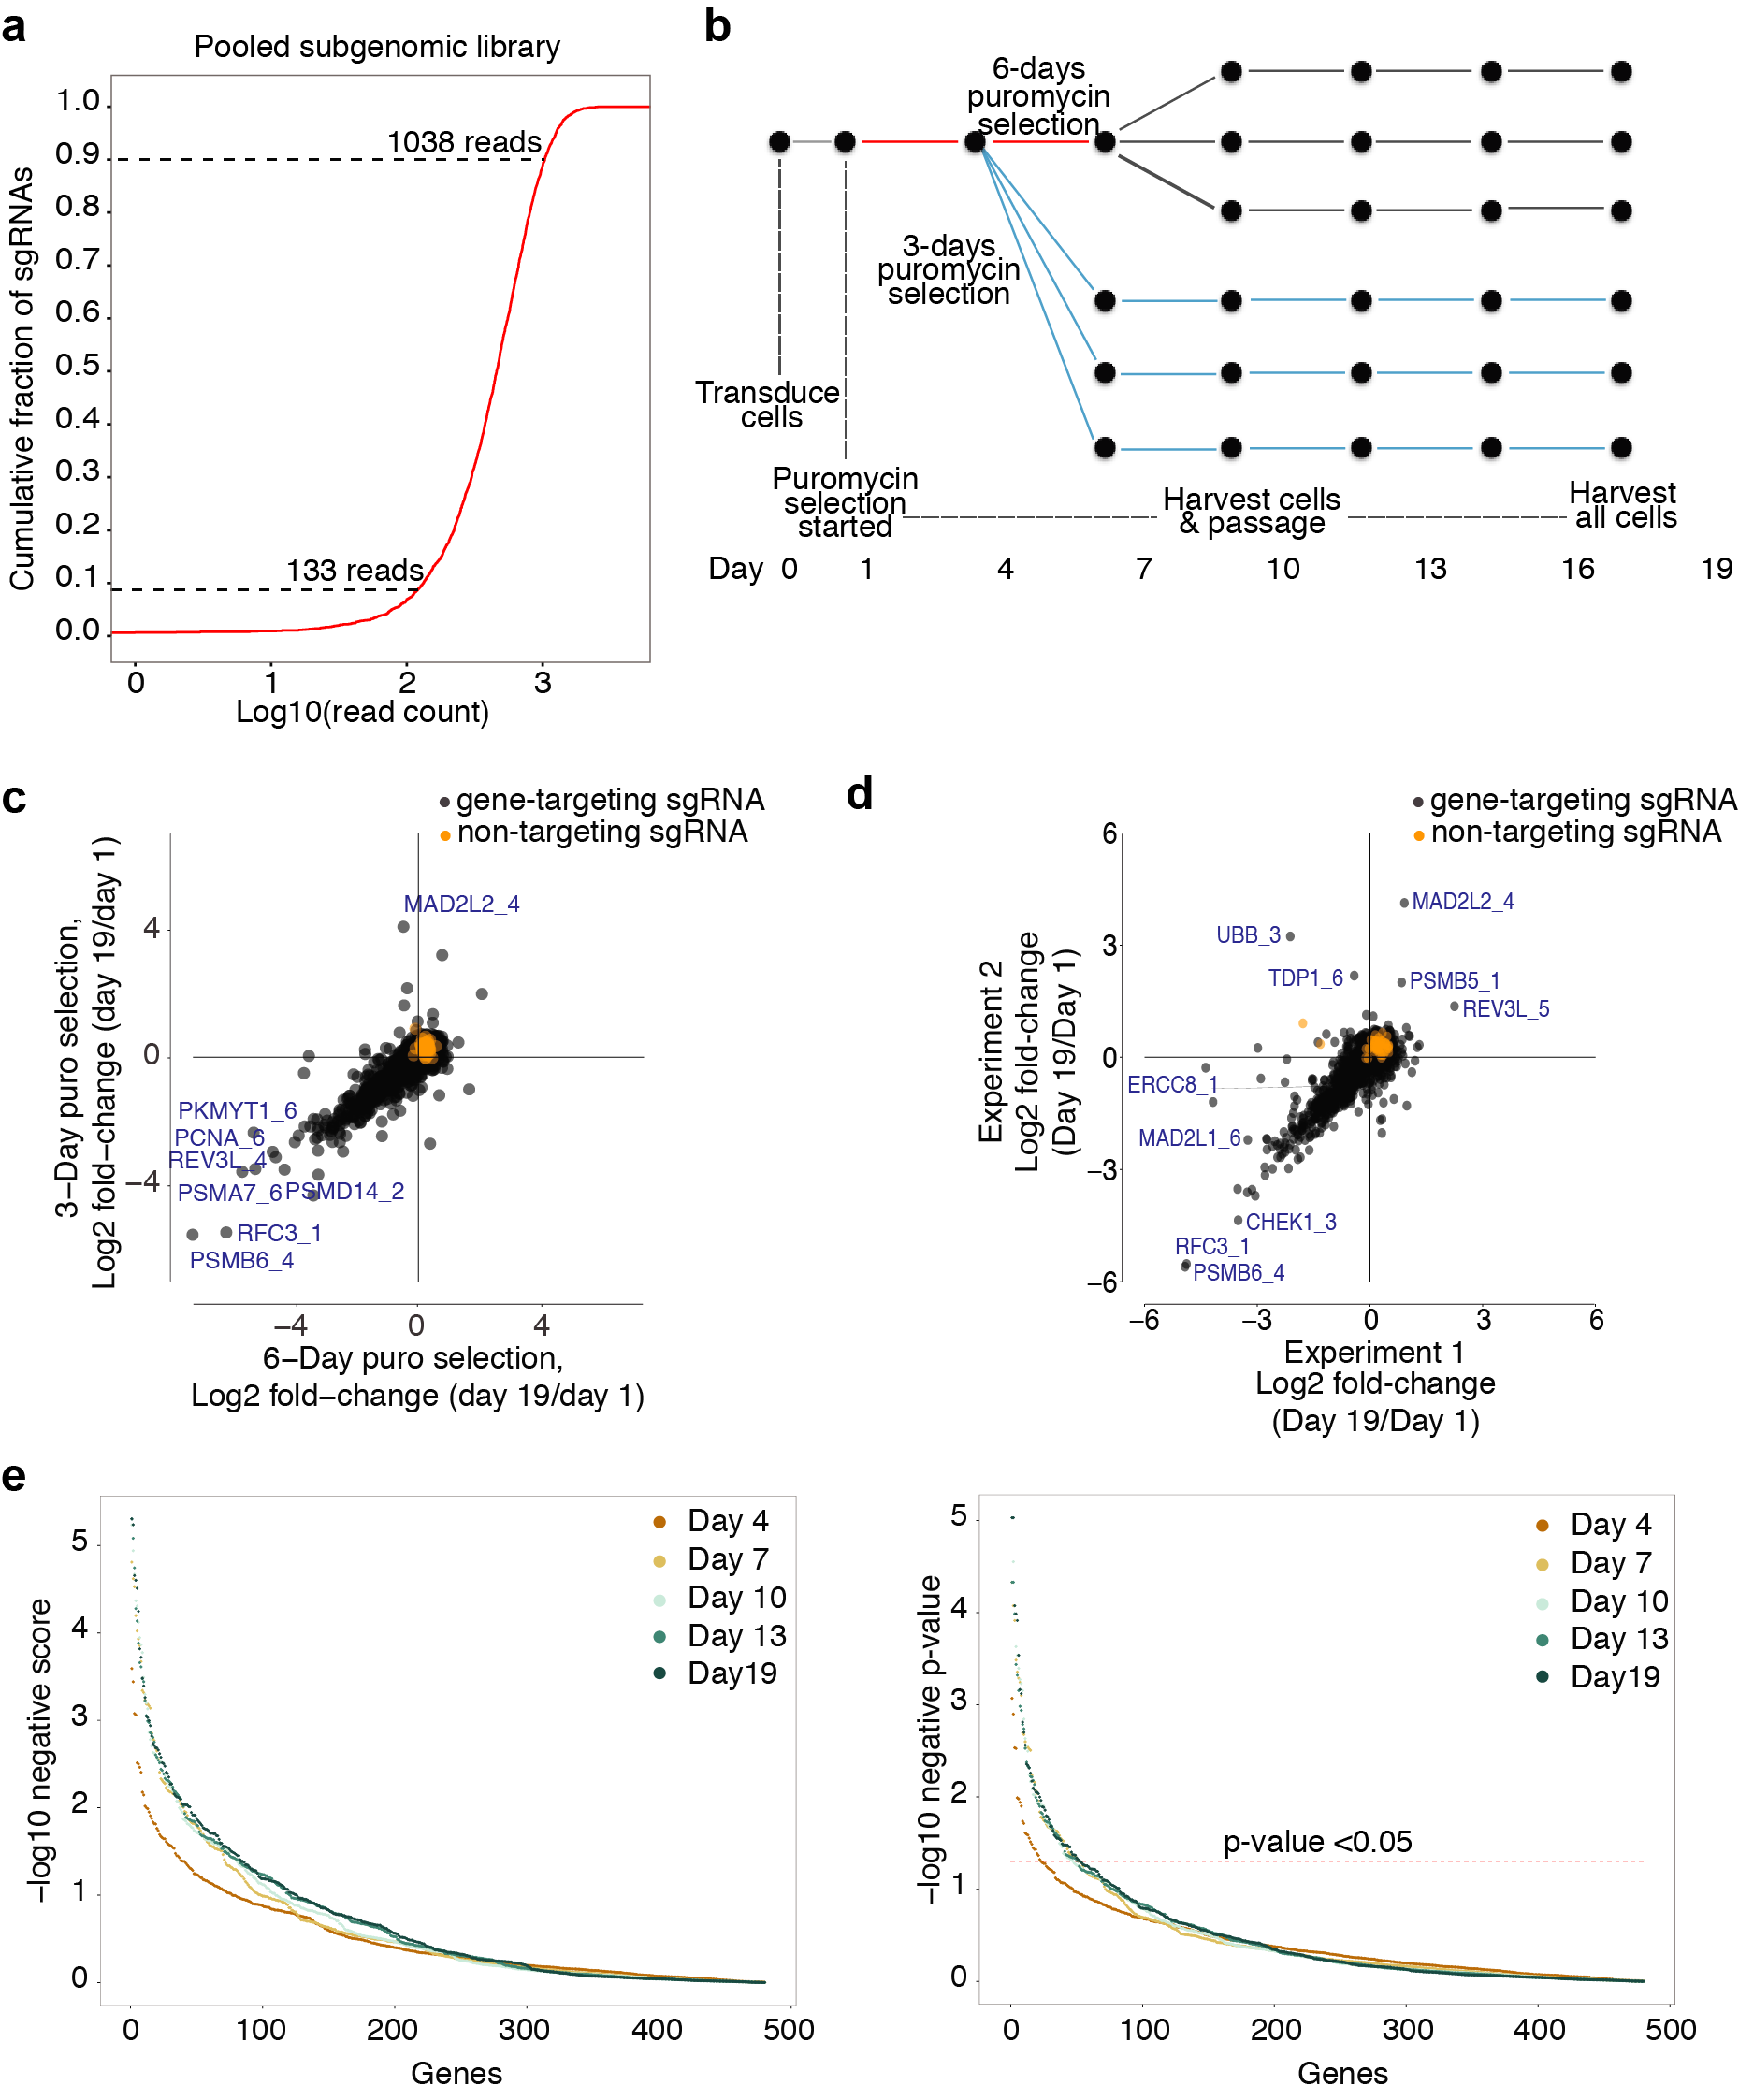
\includegraphics[width=1\textwidth]{supplement/figures/pooled_screen}
    \caption[Quality control of dropout screens]
            {\small{\textbf{Quality control analysis of pooled subgenomic library and dropout genetic screens data.}}
            }
        \label{sfig:dropout-screen}
\end{figure}

\addtocounter{figure}{-1}
\begin{figure}
  \caption{
            \newline
            \textbf{a}, Cumulative distribution of sequencing reads for all the sgRNAs in the pooled plasmid library.
            \newline
            \textbf{b}, Experimental design of dropout genetic screens.
            \newline
            \textbf{c}, Scatter plot showing log2 fold-change in normalized sgRNA counts on day 19 w.r.t. day 1 after 3-days puromycin selection versus that after 6-days puromycin selection. sgRNA counts represent means of three replicates. Non-targeting sgRNAs are shown in yellow and gene-targeting sgRNAs in black. sgRNA names showing greater than 4 or less than -4 log2 fold-change are highlighted in blue.
            \newline
            \textbf{d}, Scatter plot showing log2 fold-change in normalized sgRNA counts on day 19 w.r.t. day 1 in two independent screens with 3-days puromycin selection. sgRNA counts represent means of three replicates. Non-targeting sgRNAs are shown in yellow and gene-targeting sgRNAs in black. Some sgRNA names showing greater than 2 or less than -3 log2 fold-change are highlighted in blue.
            \newline
            \textbf{e}, Negative score and negative P-value distribution. For all the genes in the screen data (from the two independent screens with 3-days puromycin selection), the -log10 negative score (left panel) and negative P-values (right panel) as determined by MAGeCK are plotted for days 4, 7, 10, 13 and 19 w.r.t. day 1. Non-targeting sgRNAs were excluded from the analysis. Genes with P-values below the threshold ($<$0.05) are above the dotted line. 
        }
\end{figure}

\clearpage

\begin{figure}
    \centering
    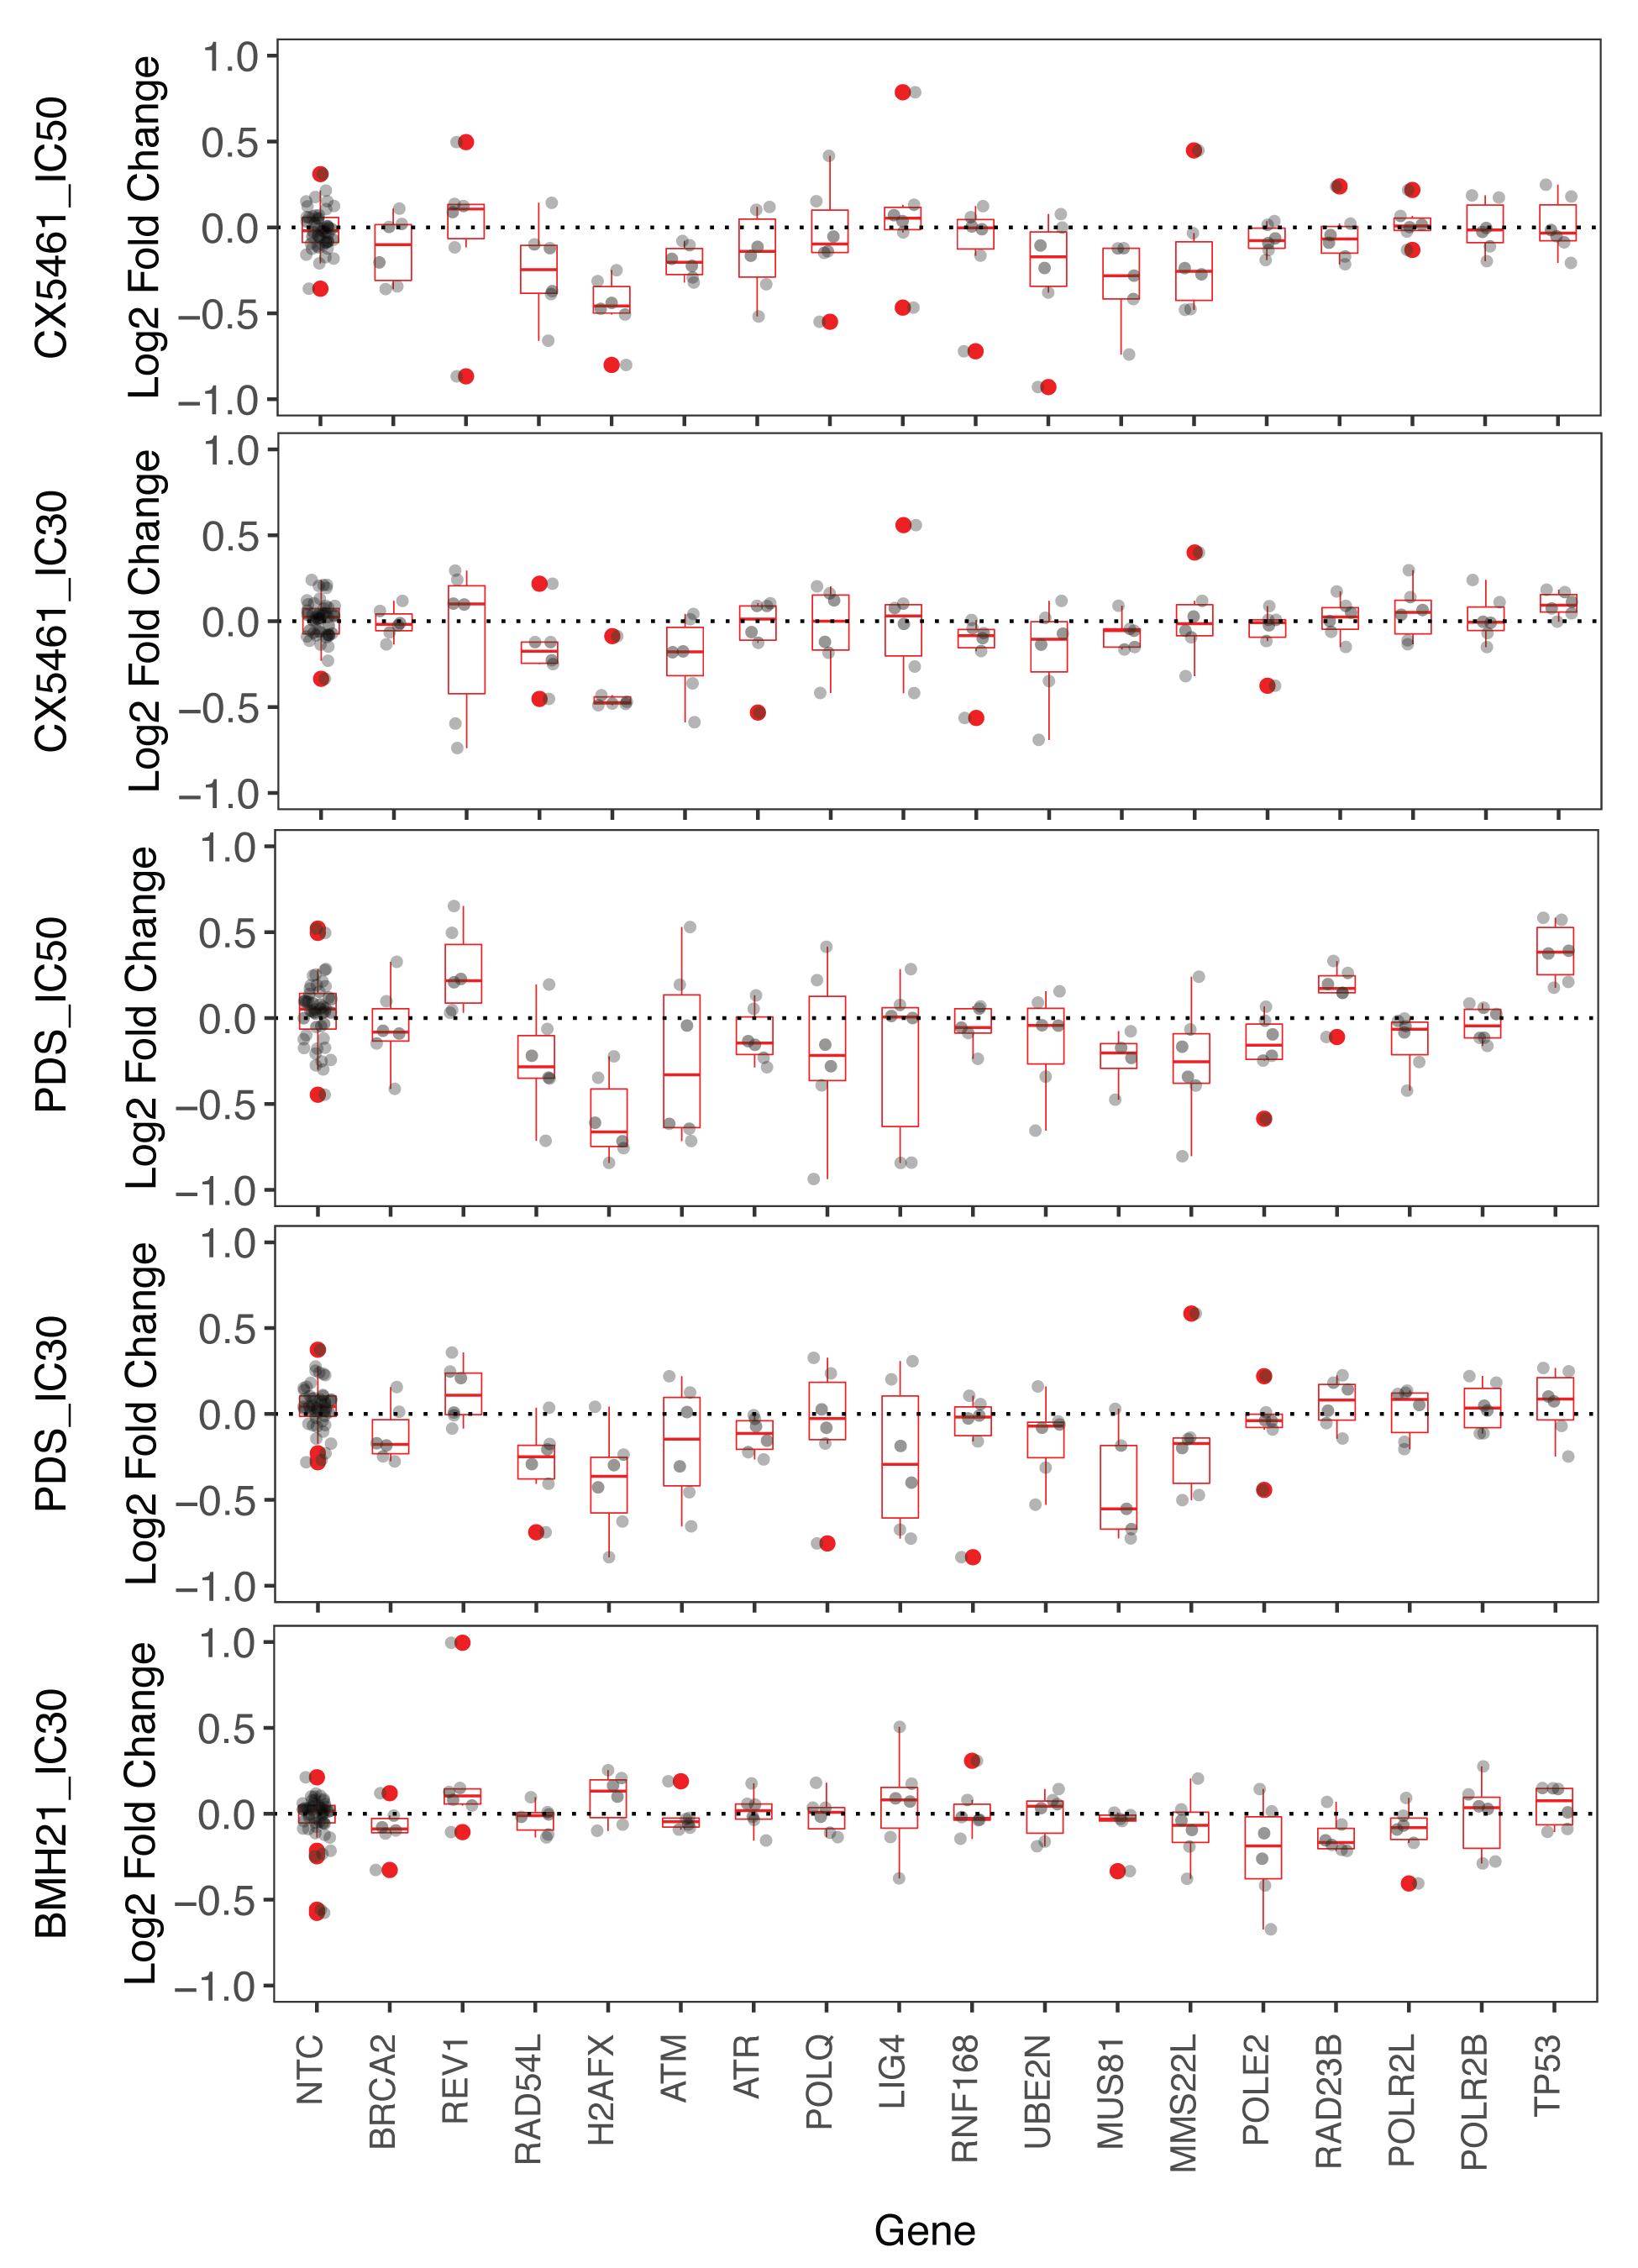
\includegraphics[width=0.8\textwidth]{supplement/figures/sgRNABoxplots}
    \caption[Individual sgRNA fold-changes of top depleted genes]
            {\textbf{Individual sgRNA fold-changes of top depleted genes.} Means of the Log2 fold-change of individual sgRNAs from the drug screen, compared with non-targeting control (NTC), following 14 day treatment with CX-5461 (IC$_{50}$ or IC$_{30}$), PDS (IC$_{50}$ or IC$_{30}$), or BMH-21 (IC$_{30}$). Dots show the Log2 fold-change of individual sgRNAs (6 per gene for gene-targeting; 50 sgRNAs total for non-targeting). Boxplot shows the distribution of the sgRNAs combined, with median shown by horizontal lines.  sgRNAs with readcounts less than 30 were filtered. sgRNAs recognized to be outliers are shown as separate circular dots.
            }
    \label{sfig:sgrna_boxplots}
\end{figure}     

\begin{figure}
    \centering
    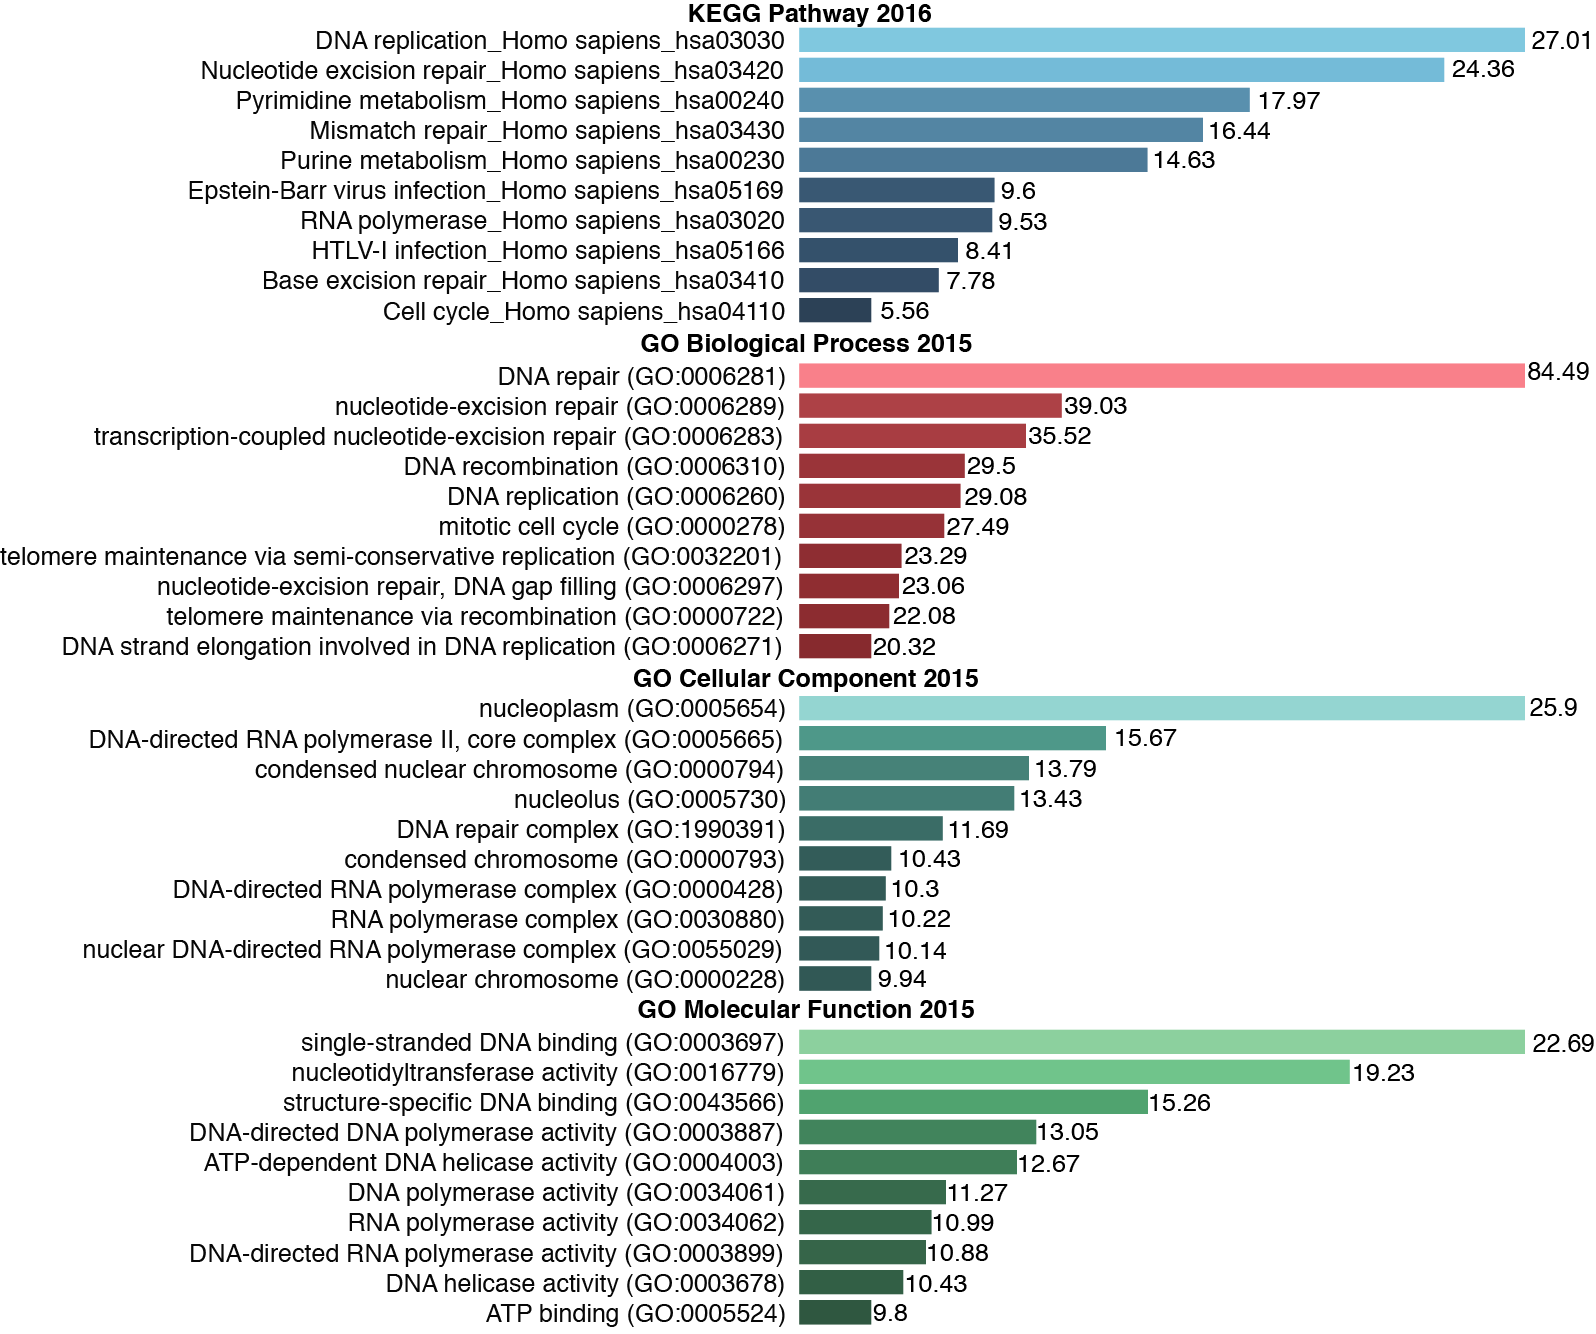
\includegraphics[width=0.8\textwidth]{supplement/figures/BMH21_Enrichr}
    \caption[KEGG pathway and Gene Ontology enrichment analysis]
            {\small{\textbf{KEGG pathway and Gene Ontology enrichment analysis for top gene hits from BMH21-treatment group.}}
            \textbf{} KEGG pathway and Gene Ontology enrichment analysis for 19 genes (P-value of $<$0.045) exclusive to BMH21 screens was performed using Enrichr. The top enriched categories are shown, ranked by the combined score (represented by the length of the bar) which is calculated using the P-value computed from Fisher exact test and z-score of the deviation from the expected rank. The brightness of the color indicates the significance. The numbers adjacent to the bars indicate the combined score.
            }
        \label{sfig:bmh21_enrichr}
\end{figure}

\begin{figure}
    \centering
    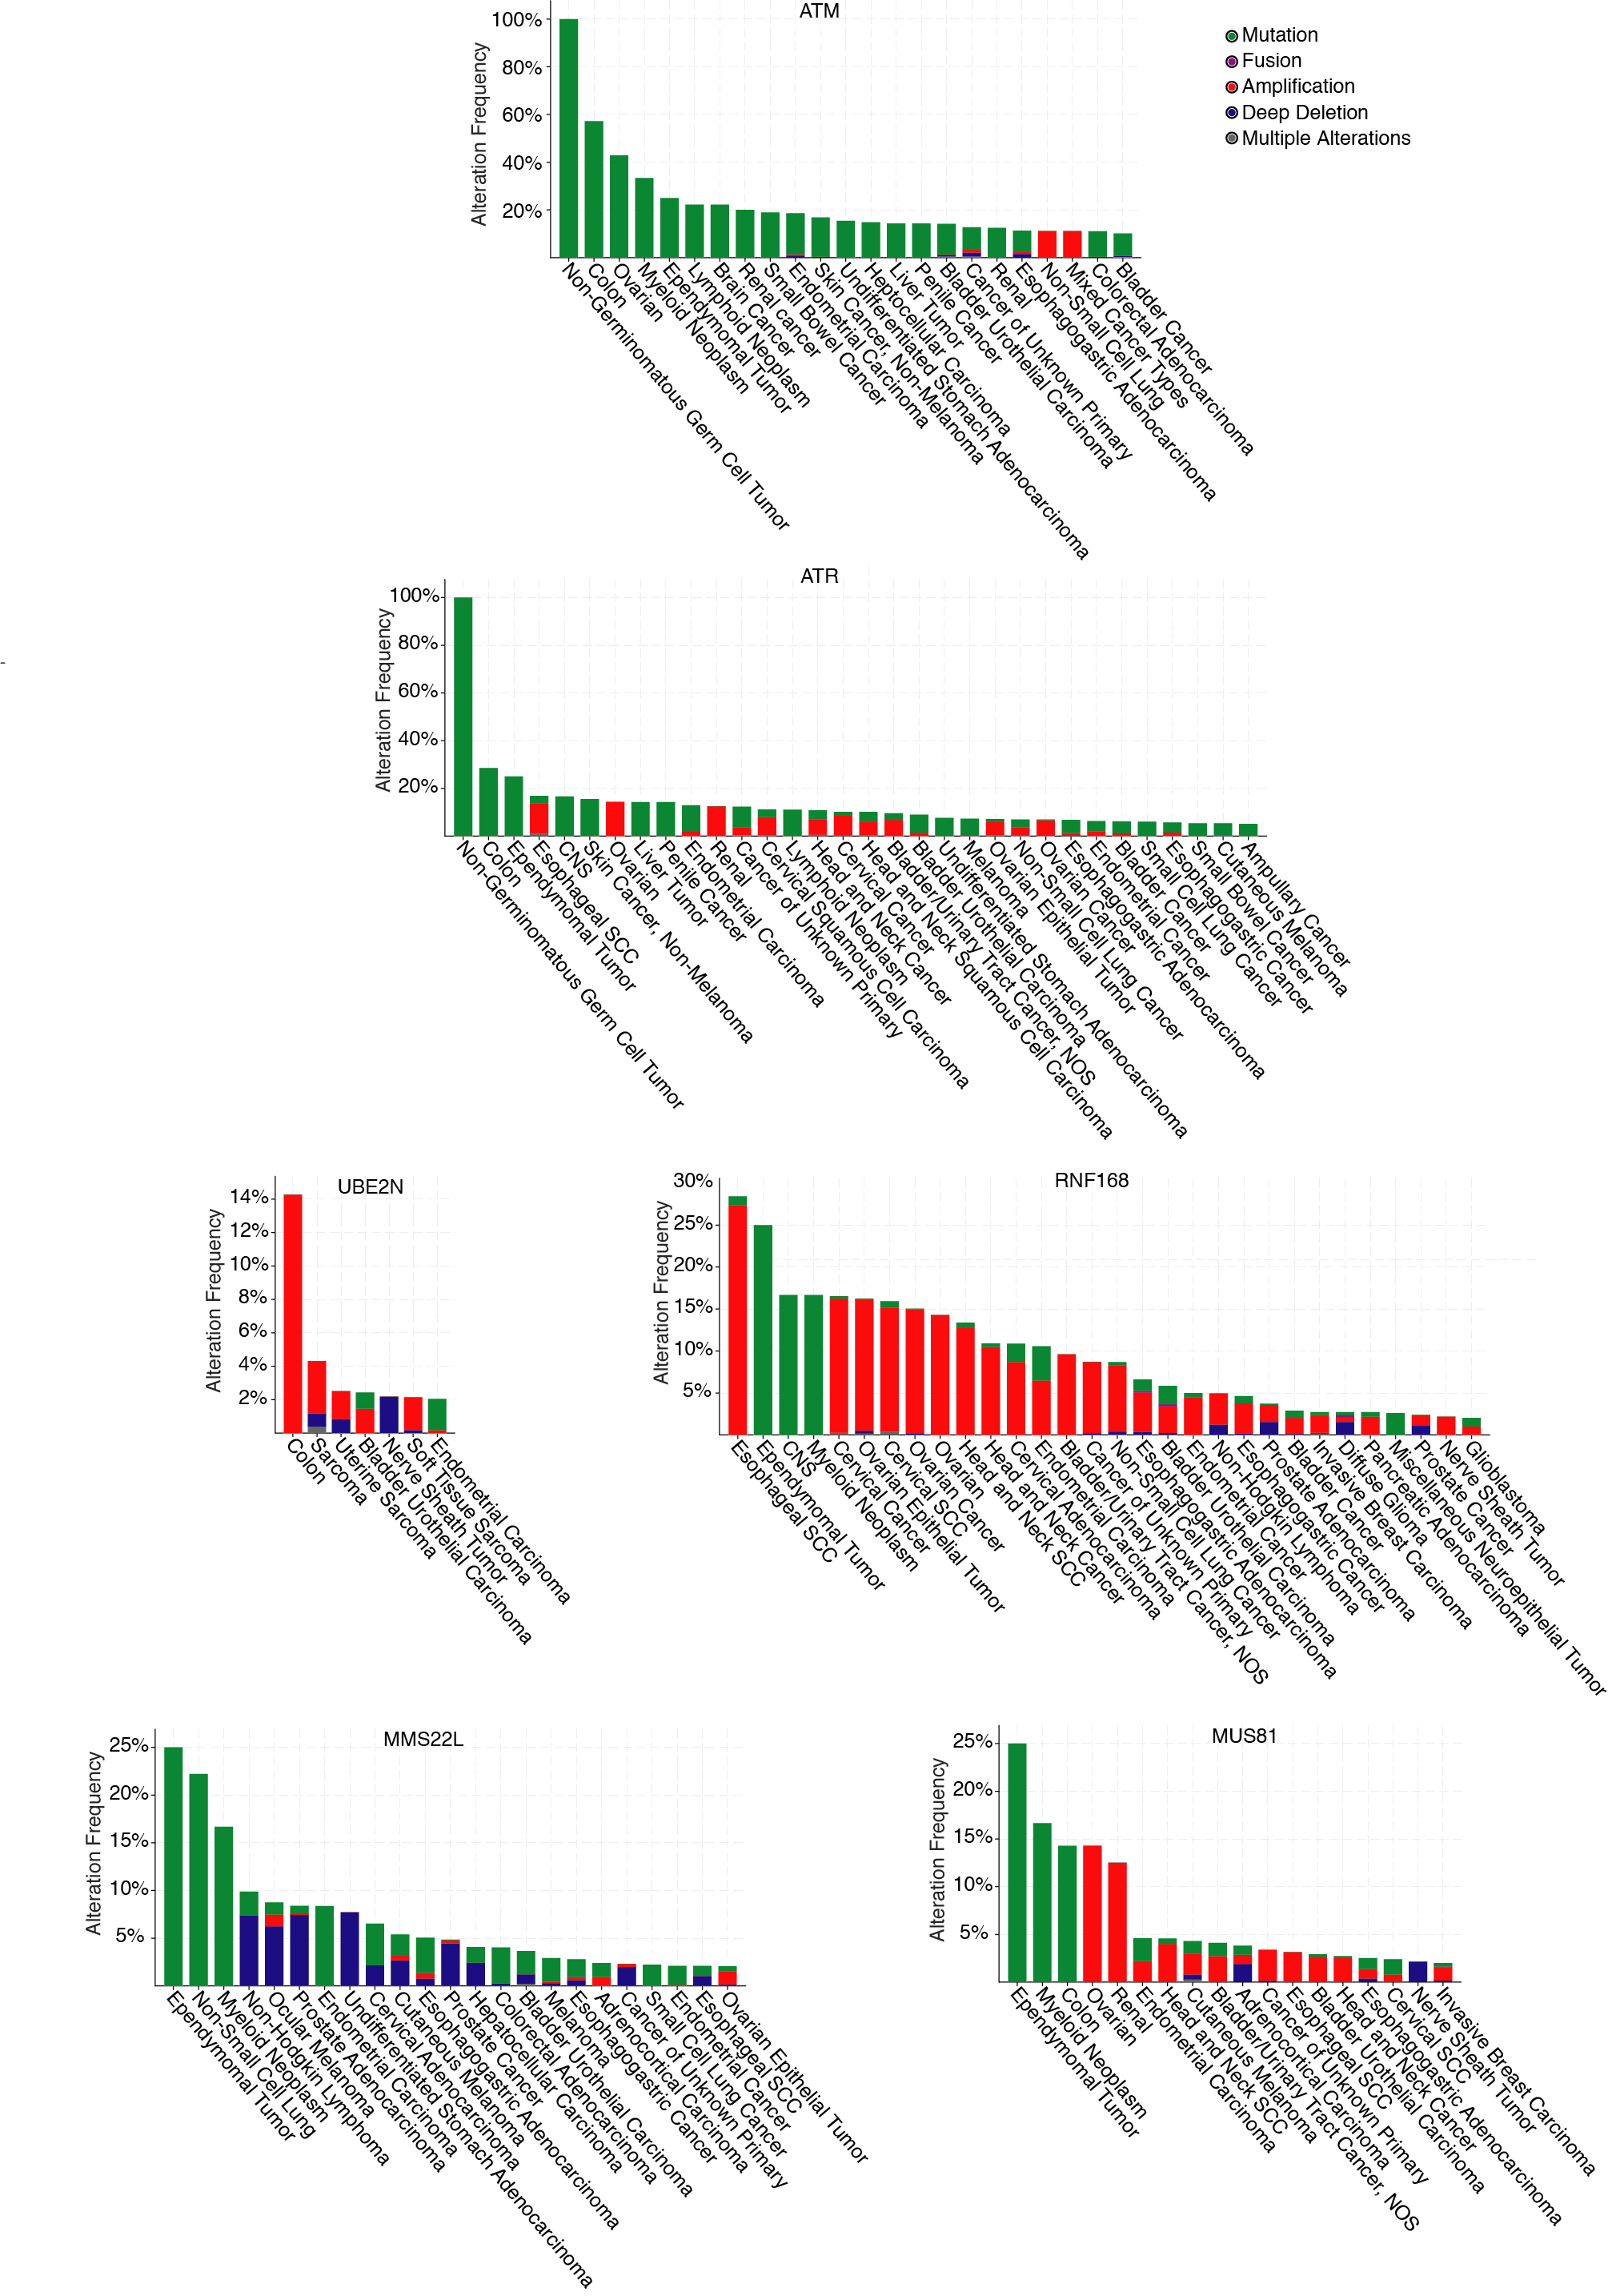
\includegraphics[width=0.8\textwidth]{supplement/figures/cbioportal}
    \caption[Cancer-associated genetic alterations in top gene hits]
            {\small{\textbf{Genetic alterations in top gene hits in different cancers types.}}
            \textbf{} Genetic alterations in genes in different cancers with a minimum of 10\% (ATM), 5\% (ATR) and 2\% (UBE2N, RNF168, MUS81, MMS22L) of altered cases in each cancer type were determined using CBioPortal database. SCC=Squamous cell carcinoma 
            }
        \label{sfig:cbioportal}
\end{figure}

\begin{figure}
    \centering
    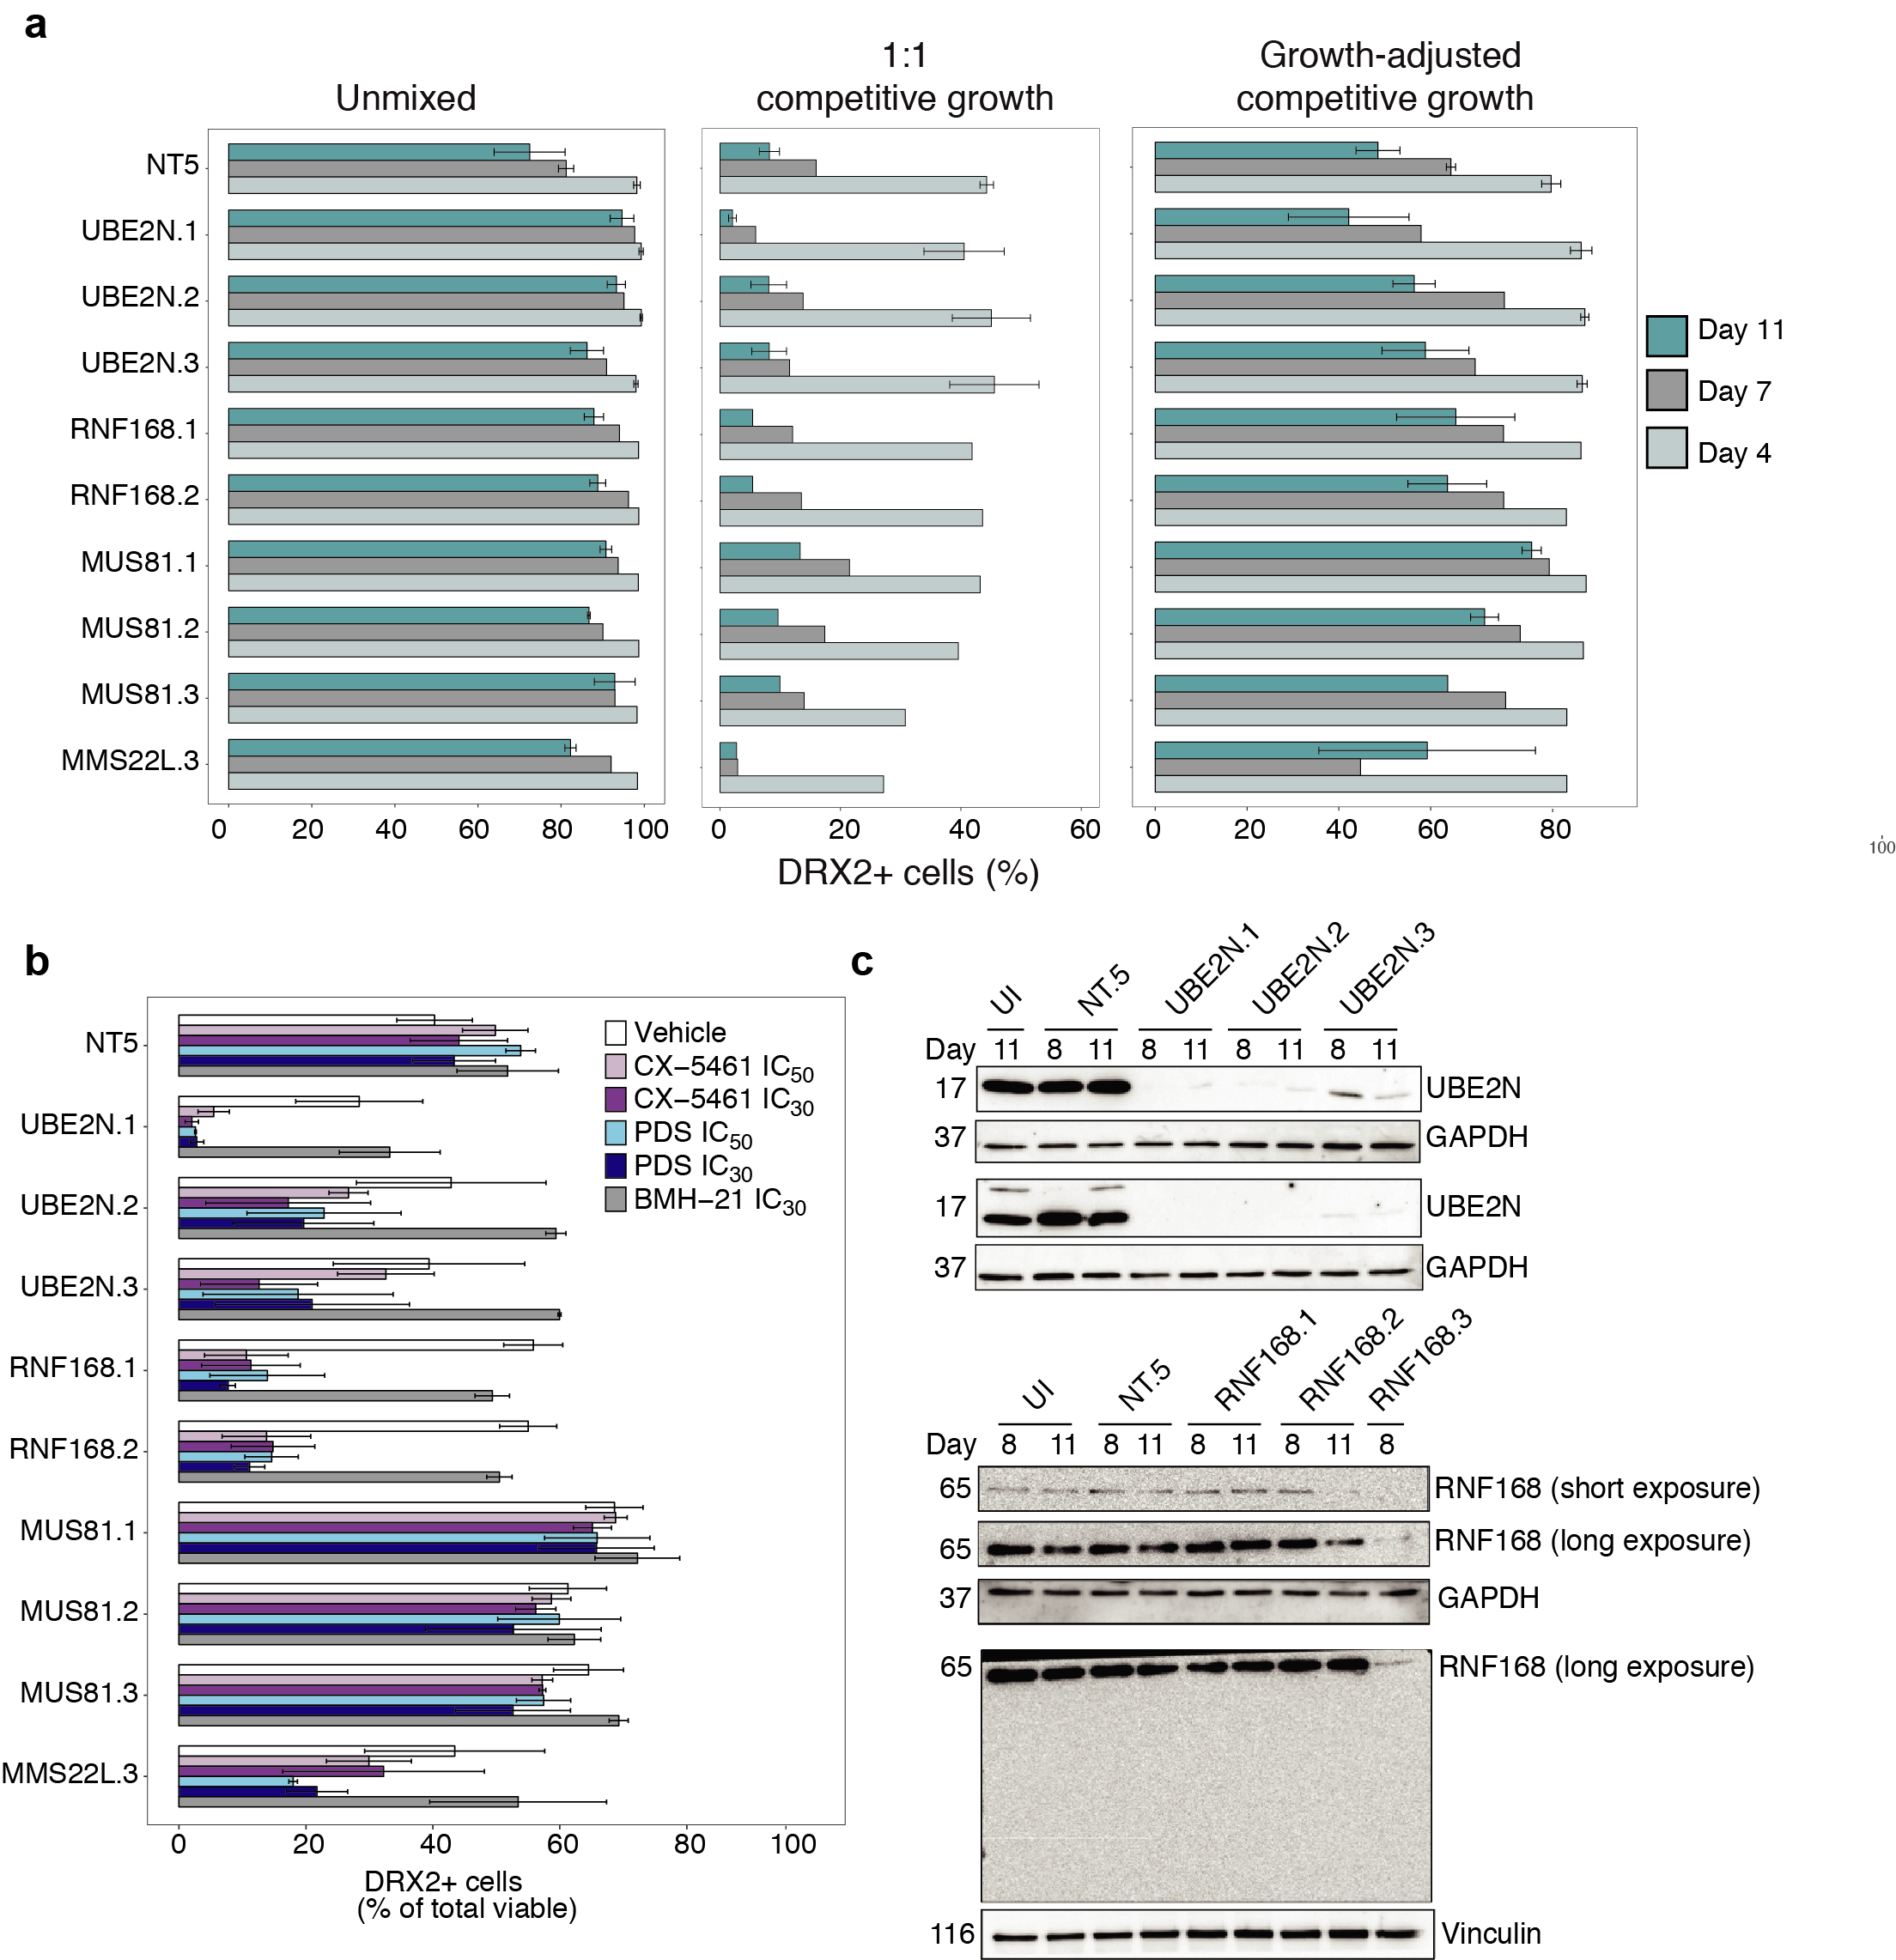
\includegraphics[width=0.9\textwidth]{supplement/figures/screen_validation}
    \caption[Gene hits validation]
            {\small{\textbf{Validation of drug screens in HCT116 cells.}}
            }
        \label{sfig:validation}
\end{figure}

\addtocounter{figure}{-1}
\begin{figure}
  \caption{
             HCT116 cells were transduced with individual sgRNAs including a non-targeting control (NT5), three targeting UBE2N, two for RNF168, three for MUS81, two for MMS22L. Flow analysis was performed on transduced cell populations at indicated days after transduction to determine the fraction of cells expressing red fluorescence in \textbf{a}, unmixed transduced cells as well as cells mixed at 1:1 or growth-adjusted ratios, and \textbf{b}, mixed transduced and non-transduced cell populations subjected to vehicle, CX-5461, PDS and BMH-21 treatments for one week at indicated doses. The mean for each treatment condition is shown (bar) for each mixed population with standard error of means (SEM).   
            \textbf{c}, The Western blots show UBE2N, RNF168 and GAPDH (input) gene expression in the uninfected (UI) or targeted cells at the indicated days. 
    }
\end{figure}

\clearpage

\begin{figure}
    \centering
    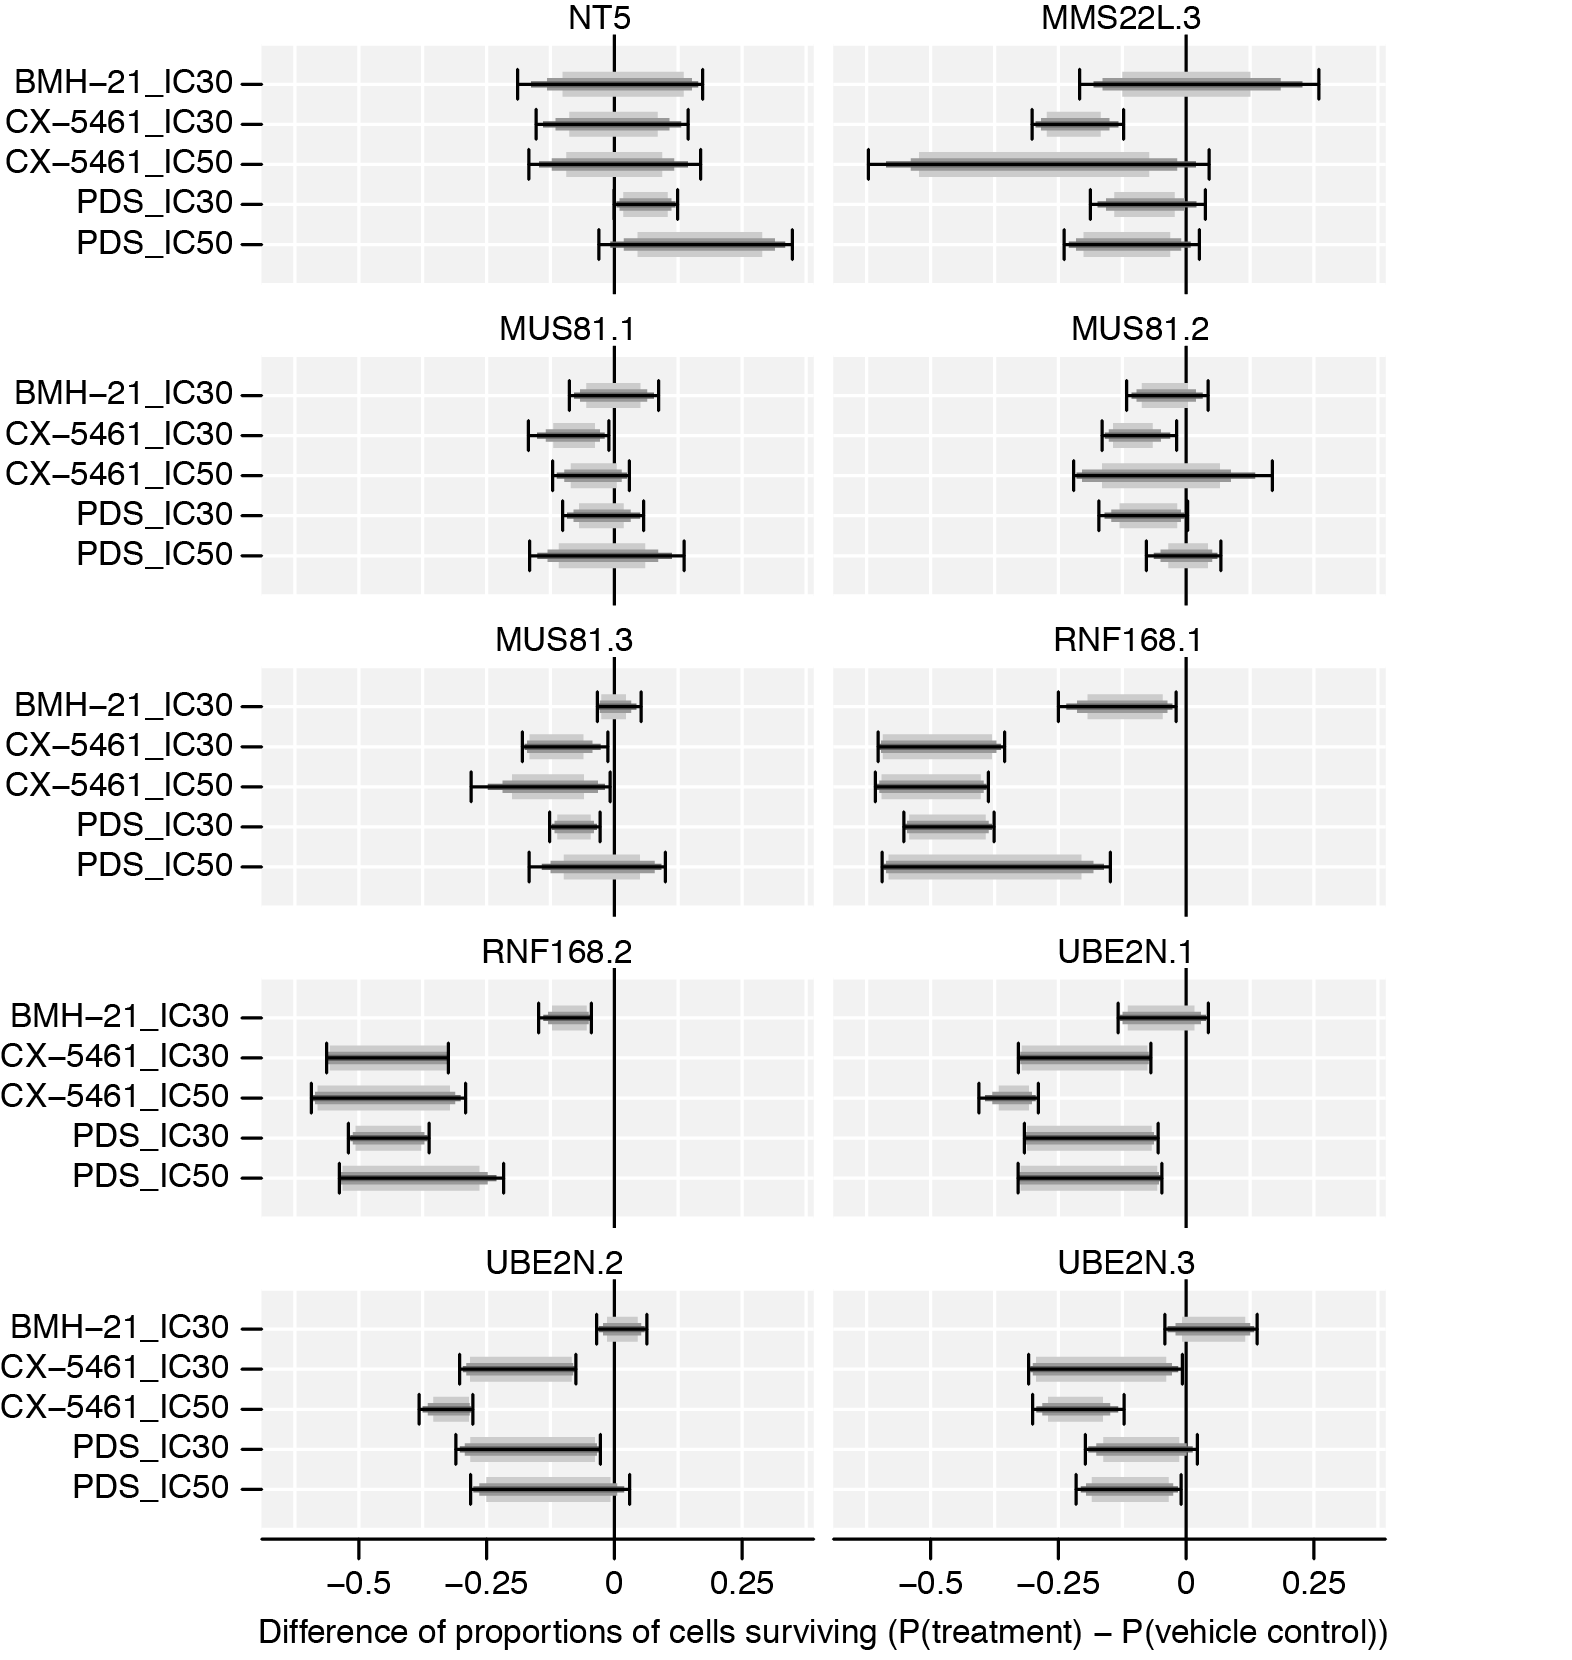
\includegraphics[width=0.8\textwidth]{supplement/figures/validation_bootstrap.png}
    \caption[CGA with confidence intervals]
            {\small{\textbf{Confidence intervals for CGA.}}
            For the CGA assay, statistical analysis was performed for each sgRNA by bootstrapping (see Methods). The x-axis indicates the confidence intervals and y-axis shows different treatment groups. The four confidence intervals are portrayed as: 95\% CI as very wide light grey box (relative width 8), 99\% CI as wide grey box (width 4), 99.9\% CI as narrow dark grey box (width 2), and 99.99\% CI as black line with end caps (width 1).
            }
        \label{sfig:validationCI}
\end{figure}

\begin{figure}
    \centering
    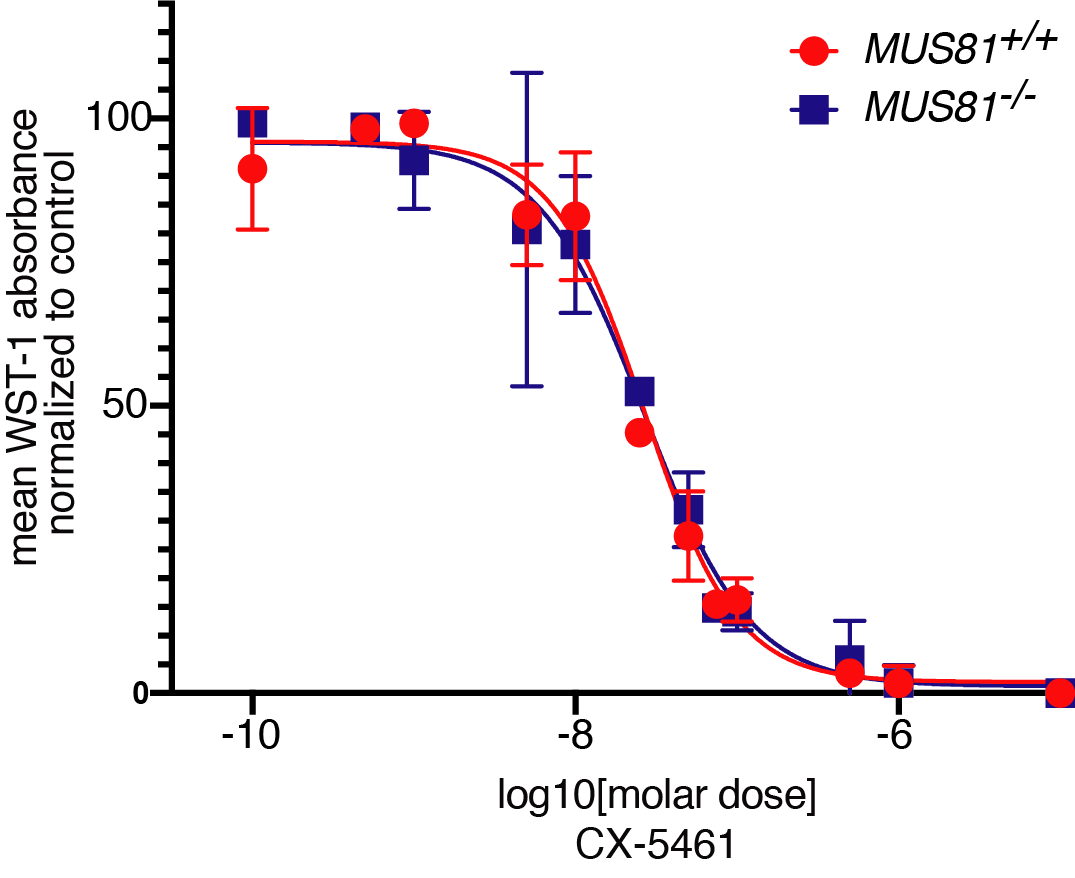
\includegraphics[width=0.8\textwidth]{supplement/figures/Mus81_cells.png}
    \caption[CX-5461 drug dose response in HCT116 MUS81-wildtype and -null cells]
            {\small{\textbf{CX-5461 drug dose response in MUS81-wildtype and -null cells.}}
            \textit{MUS81$^{+/+}$} and \textit{MUS81$^{-/-}$} HCT116 cells were treated with the vehicle or CX-5461 for 6 days and mean WST-1 absorbance was determined. 
            }
        \label{sfig:mus81cells}
\end{figure}

\begin{figure}
    \centering
    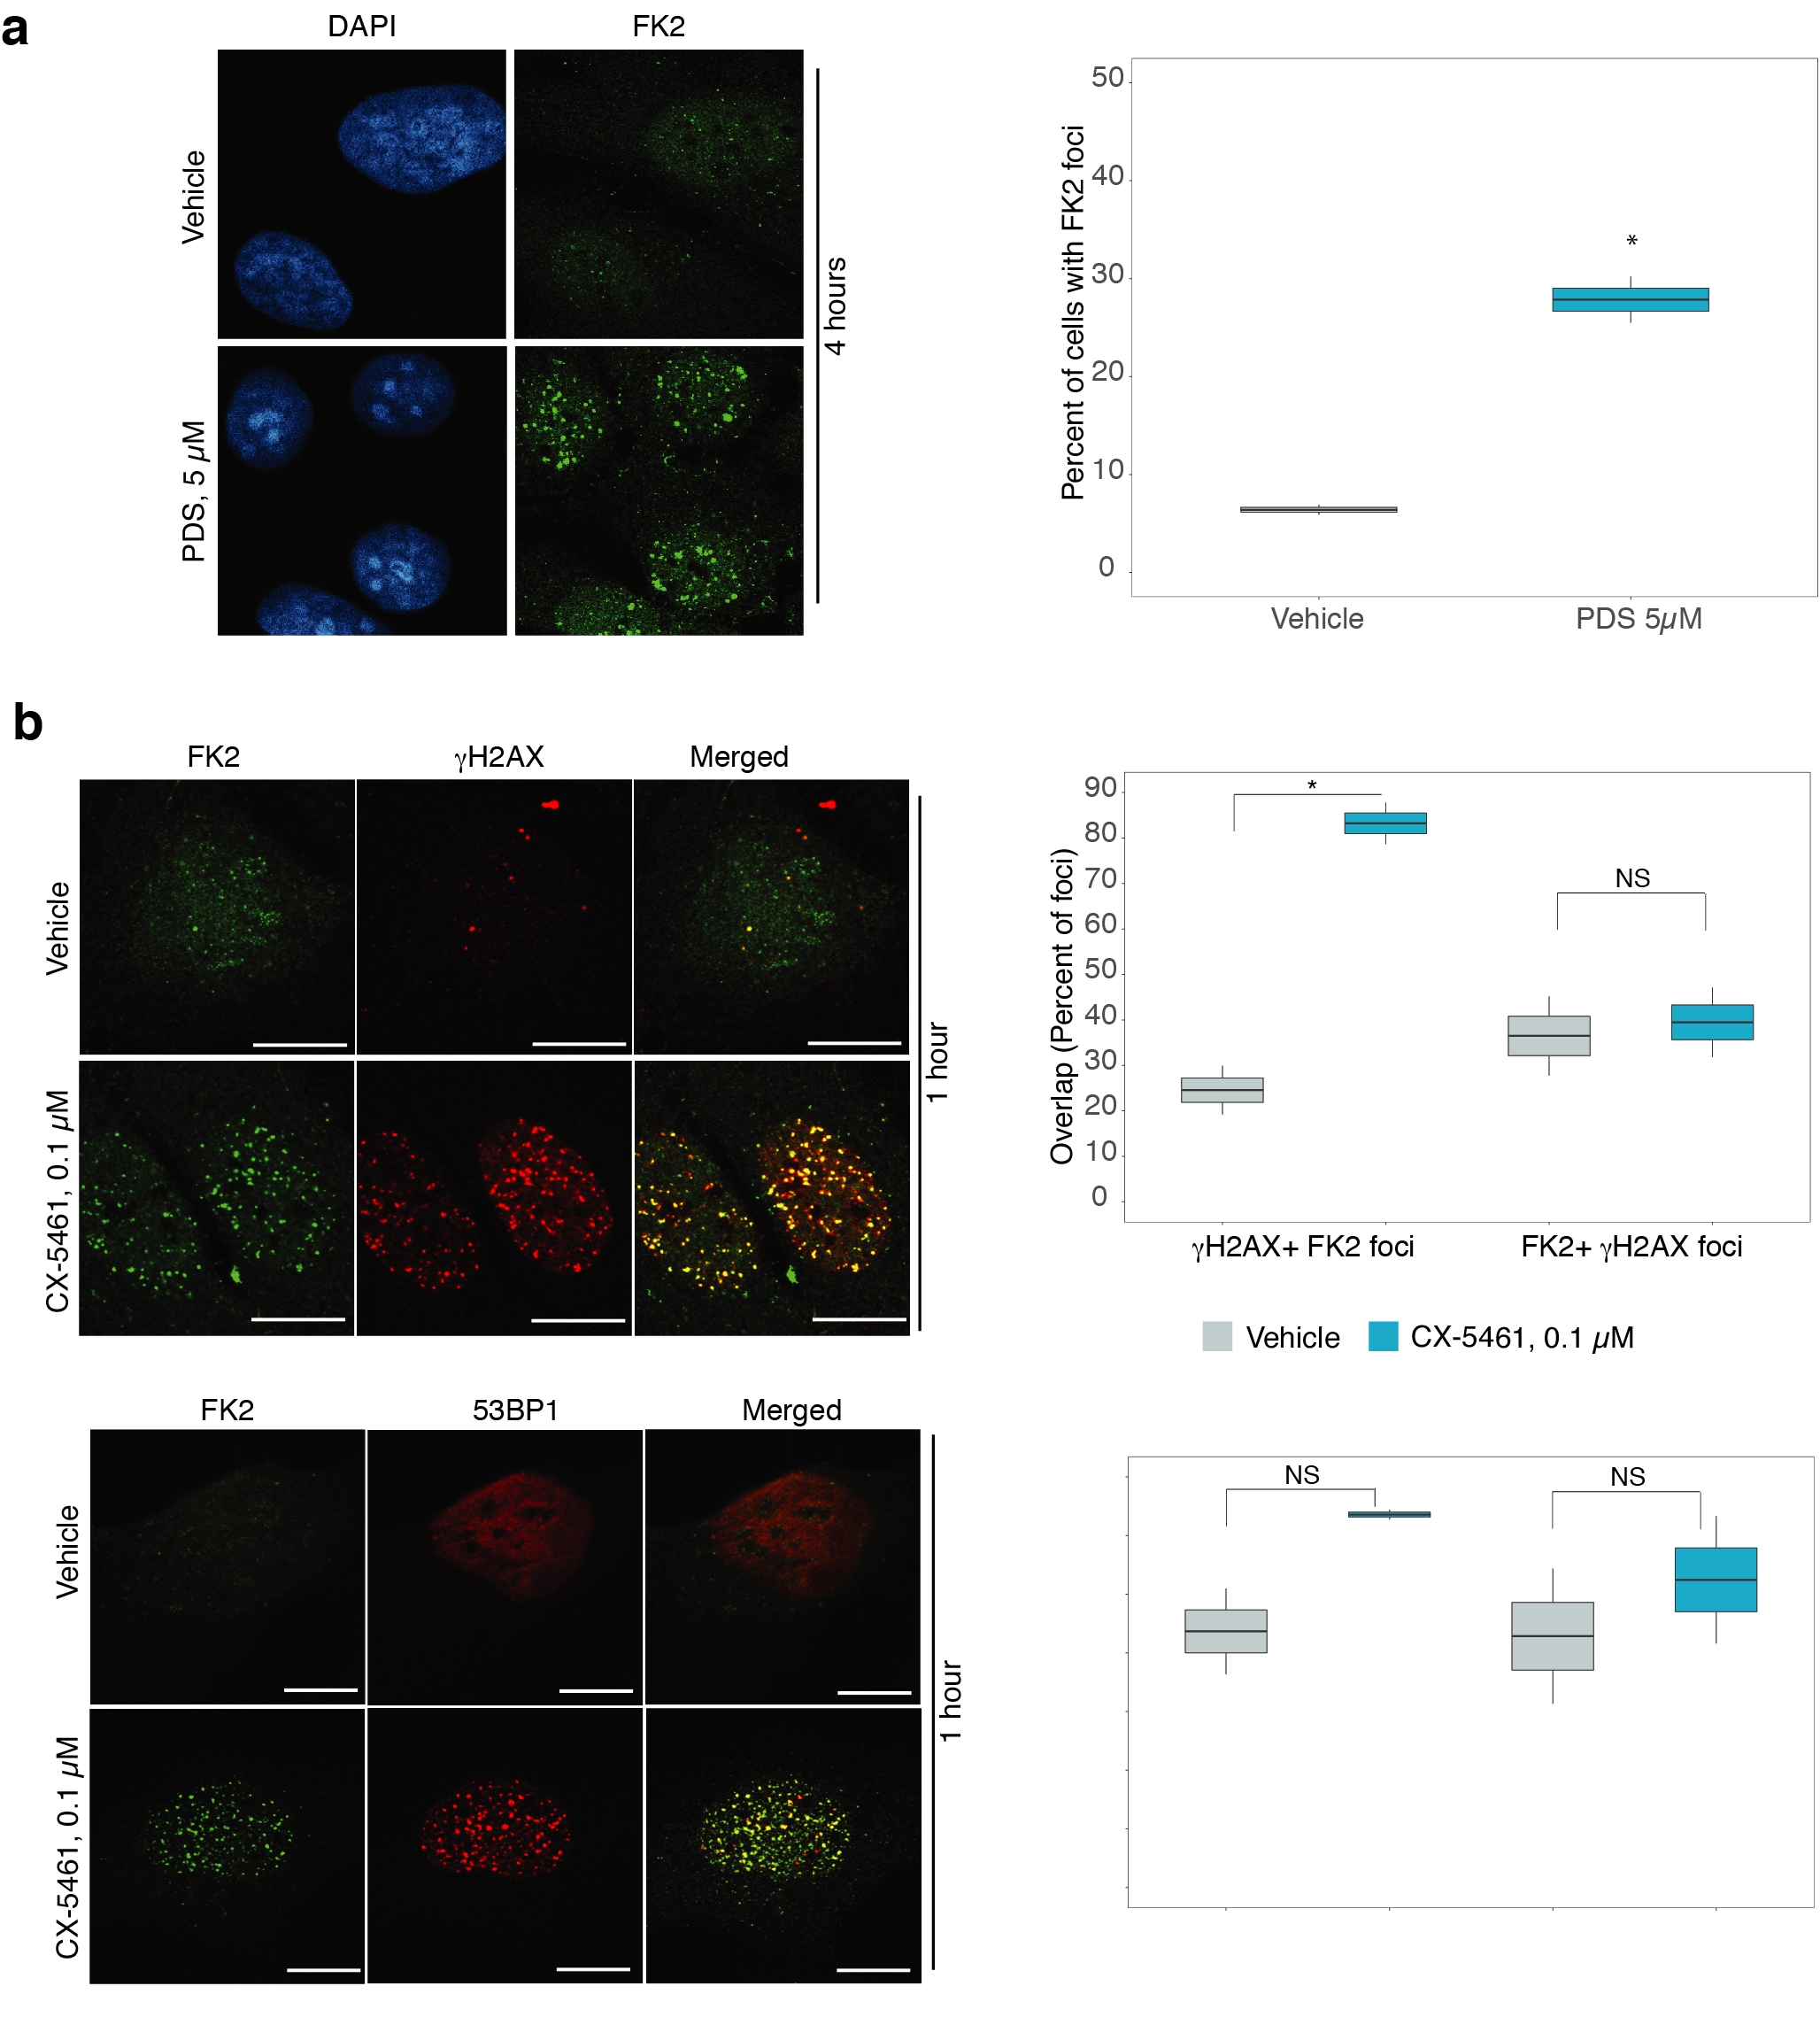
\includegraphics[width=0.8\textwidth]{supplement/figures/Ub_signaling_foci.png}
    \caption
            {\textbf{a}, FK2 foci were induced in U2OS cells after vehicle and PDS treatments at the indicated dose. Left panel shows the images of FK2 and DAPI staining. Right panel shows that the percent of cells with FK2 foci after CX-5461 is significantly higher than after vehicle treatment (* P-value$<$0.01, one-tailed unpaired t-test).  
            \newline
            \textbf{b}, FK2 foci co-localize with $\gamma$H2AX (top panel) and 53BP1 (bottom panel) DNA damage foci  after one hour of treatment with \SI{0.1}{\micro\Molar} CX-5461 in U2OS cells. * P-value$<$0.01, NS = not significant. 
            }
        \label{sfig:ub-signaling}
\end{figure}

\begin{figure}
    \centering
    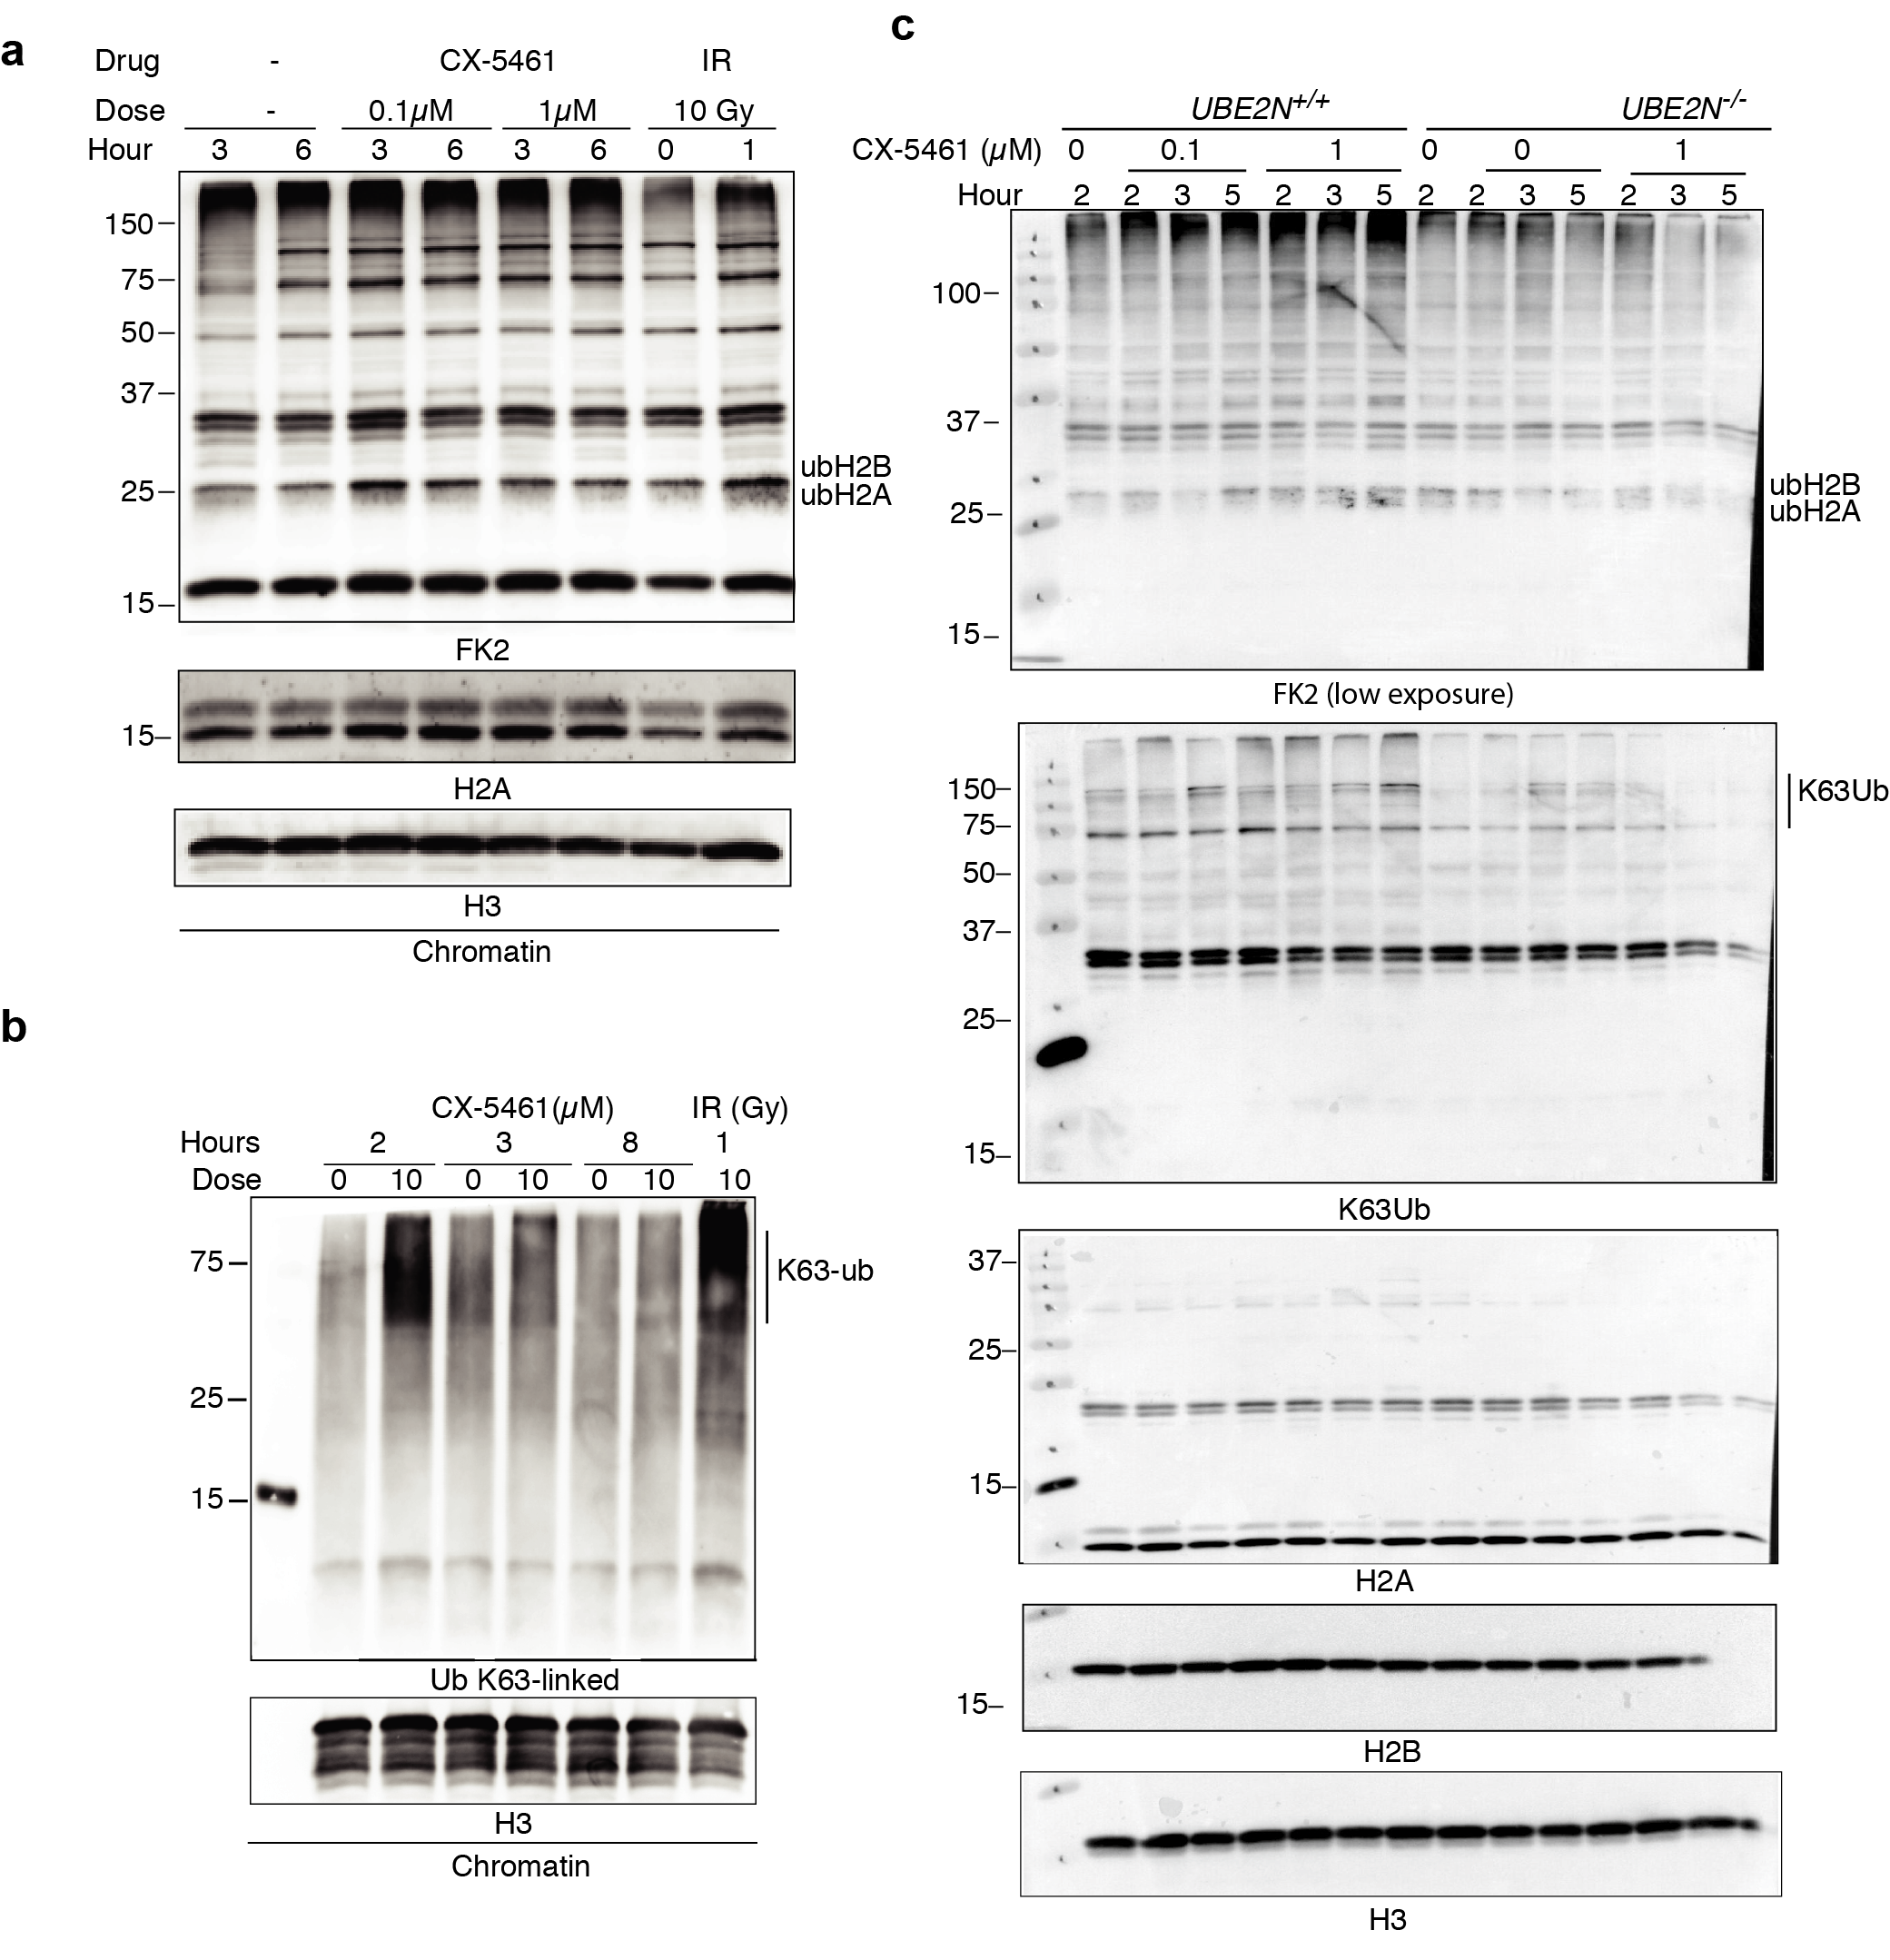
\includegraphics[width=1\textwidth]{supplement/figures/chromatin_ub_westerns}
    \caption[CX-5461-induced chromatin ubiquitination]
            {\small{\textbf{CX-5461 induces DDR-associated chromatin ubiquitination.}}
            \textbf{a, b, c}, \textit{UBE2N$^{+/+}$} (\textbf{a, b}) and \textit{UBE2N$^{-/-}$} (\textbf{c}) HCT116 cells were treated with either vehicle or CX-5461 at indicated doses and time periods, and chromatin fractions were extracted. Chromatin ubiquitination was examined using Western blots with antibodies against conjugated ubiquitin (FK2), K63-linked ubiquitin (K63Ub), histones H2A, H2B and H3. Molecular weight markers (KDa) are shown on the left. 
            }
        \label{sfig:chromatin_ub_westerns}
\end{figure}

\begin{figure}
    \centering
    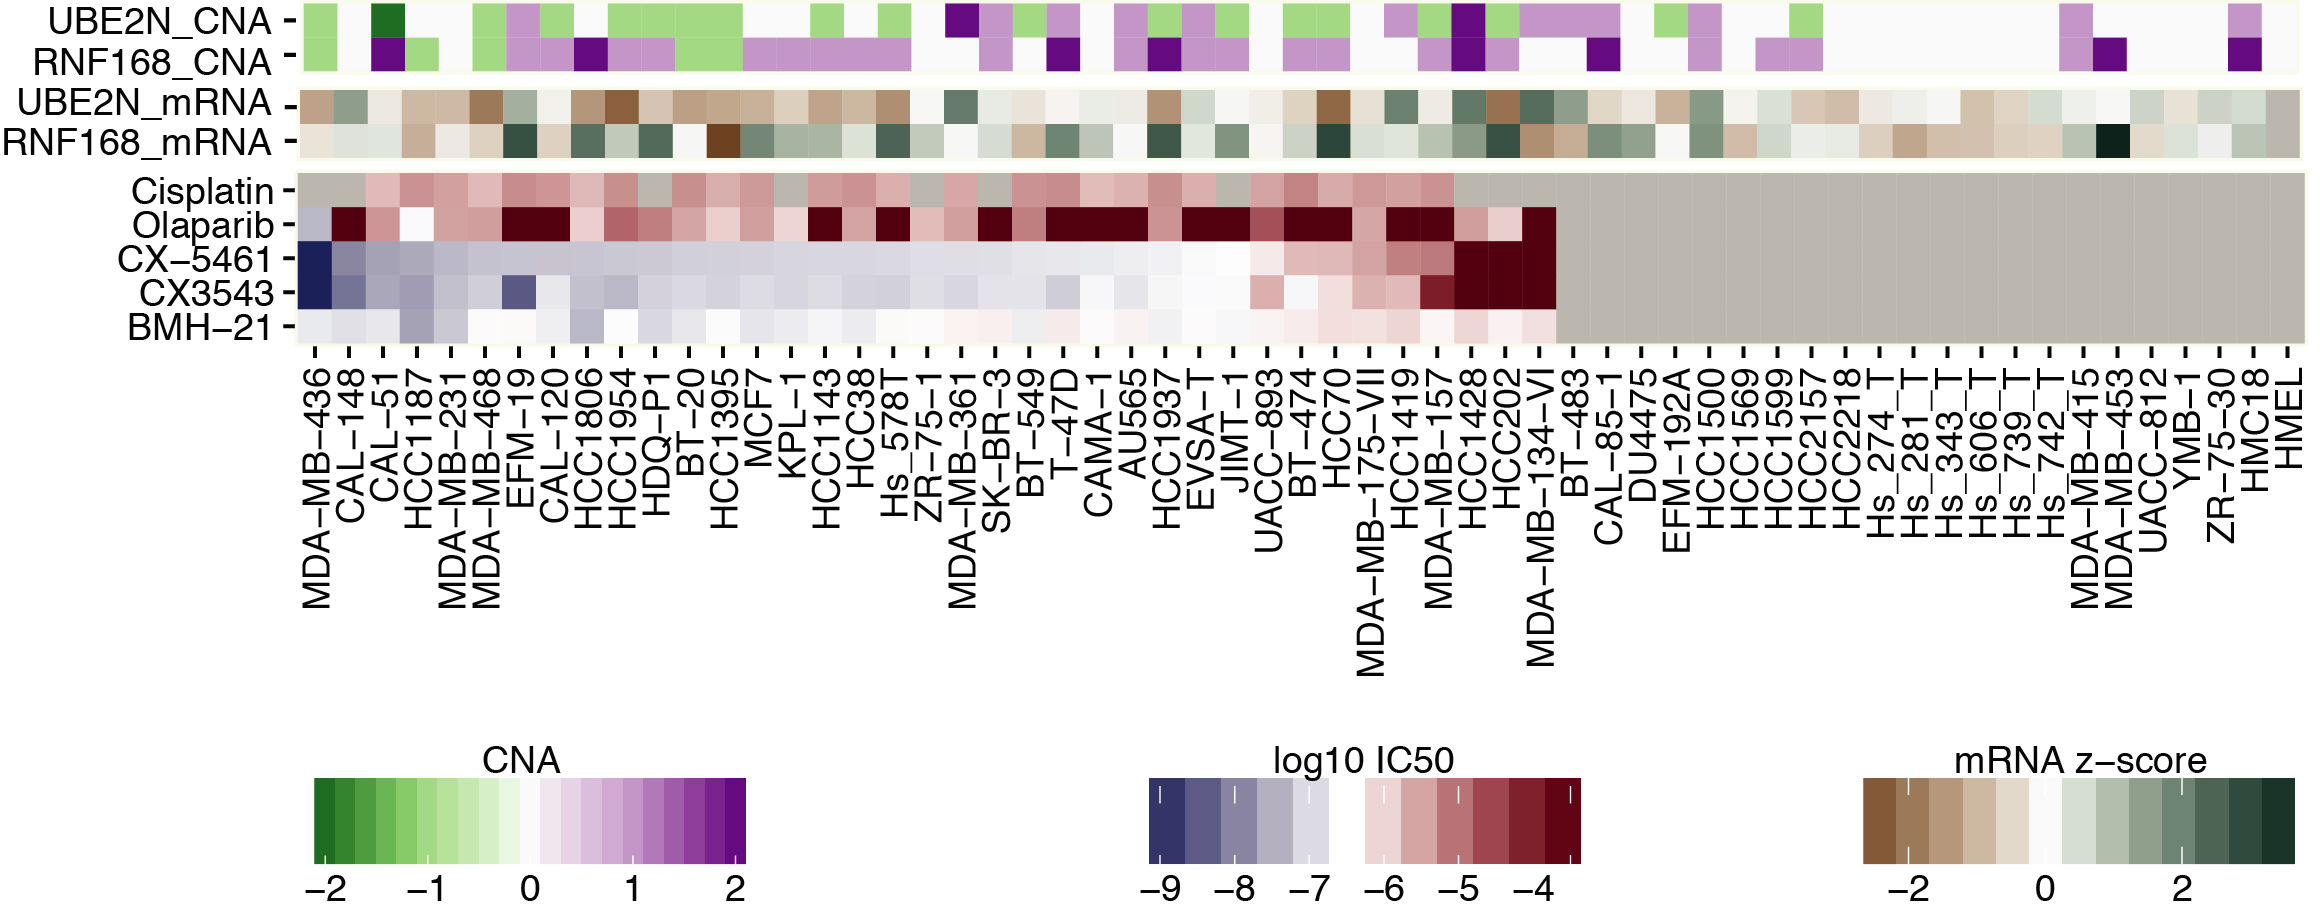
\includegraphics[width=1\textwidth]{supplement/figures/cell_lines_sensitivity.png}
    \caption[Sensitivity of breast cancer cell lines to CX-5461]
            {\small{\textbf{UBE2N and RNF168 copy number alterations (CNA) and mRNA expression, and sensitivity of breast cancer cell lines to multiple drugs.}}
            Drug sensitivity data, represented as log10 IC$_{50}$, was previously published\cite{Xu2017}. Gene copy number alterations (CNA) and mRNA (RNAseq) median z-score data was extracted from Cancer Cell Line Encyclopedia\cite{Barretina2012}.  
            }
        \label{sfig:cell_line_sensitivity}
\end{figure}

\begin{table}
\caption{Comparison of Top 10\% Depleted Genes with Hart \textit{et al}. Fitness Genes with Bayes Factor (BF).}
\centering
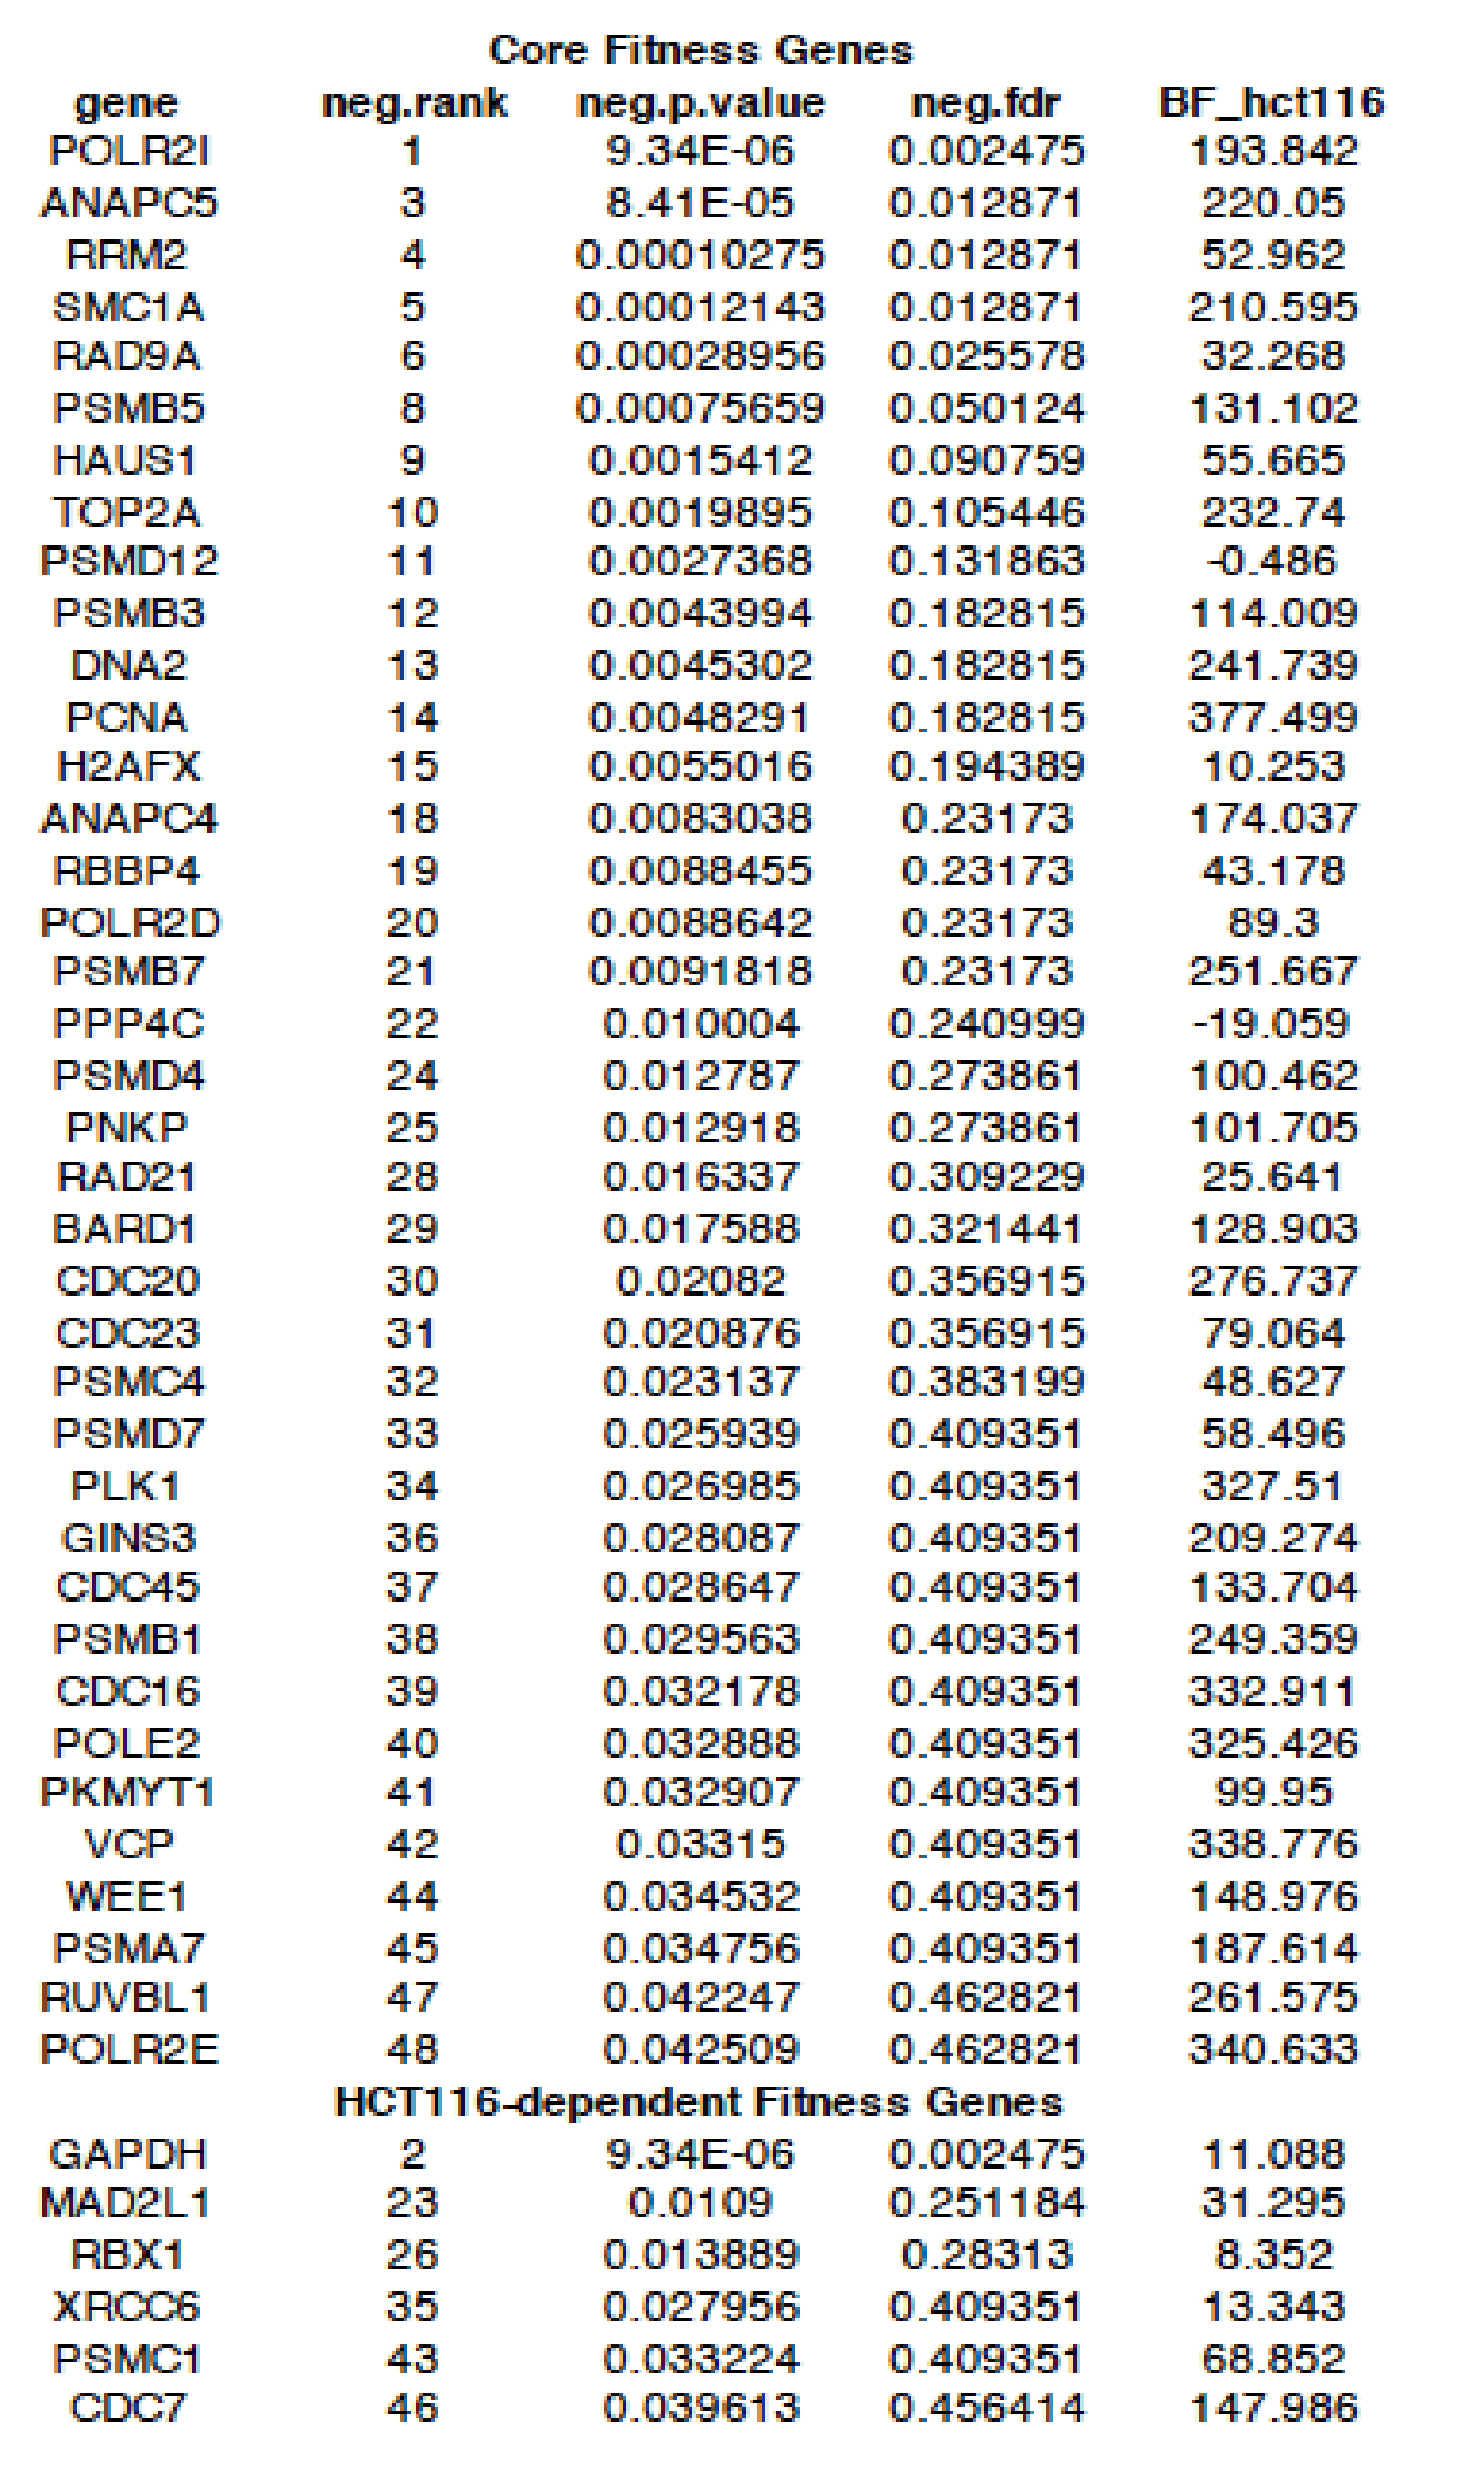
\includegraphics[width=0.8\textwidth]{supplement/tables/fitness_genes_depleted.png}
\label{table:fitness_genes}
\end{table}

\begin{table}
\caption{sgRNA Sequences Used for Genetic Validation.}
\centering
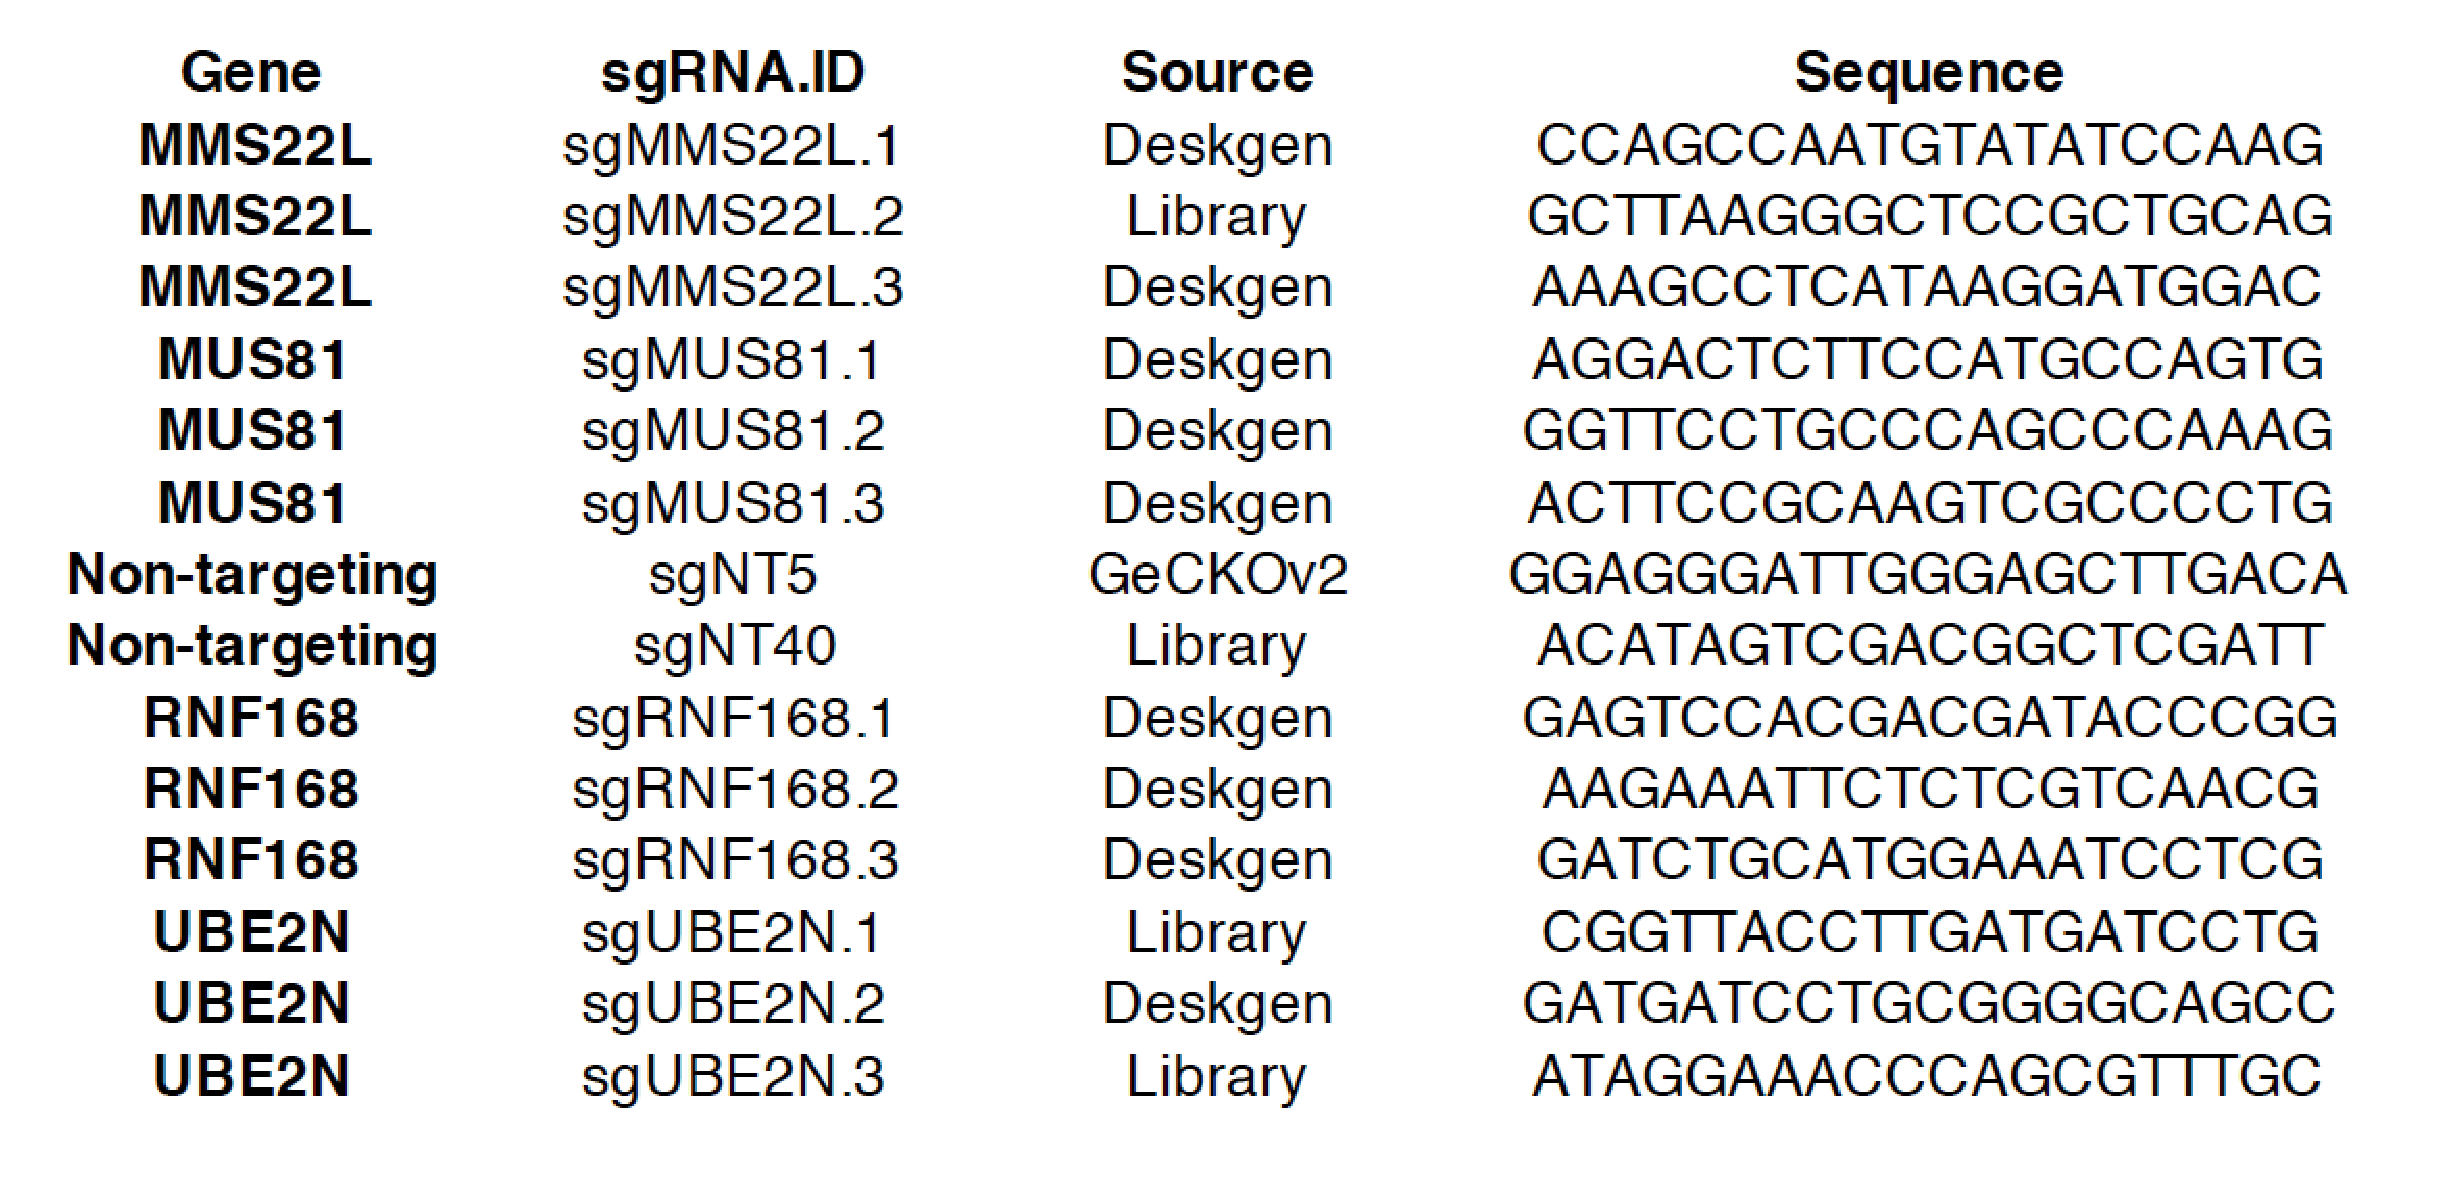
\includegraphics[width=1\textwidth]{supplement/tables/STable_sgRNA_sequences}
\label{table:sgRNA_sequences}
\end{table}

\begin{table}
\caption{Antibodies Used for Western Blots.}
\centering
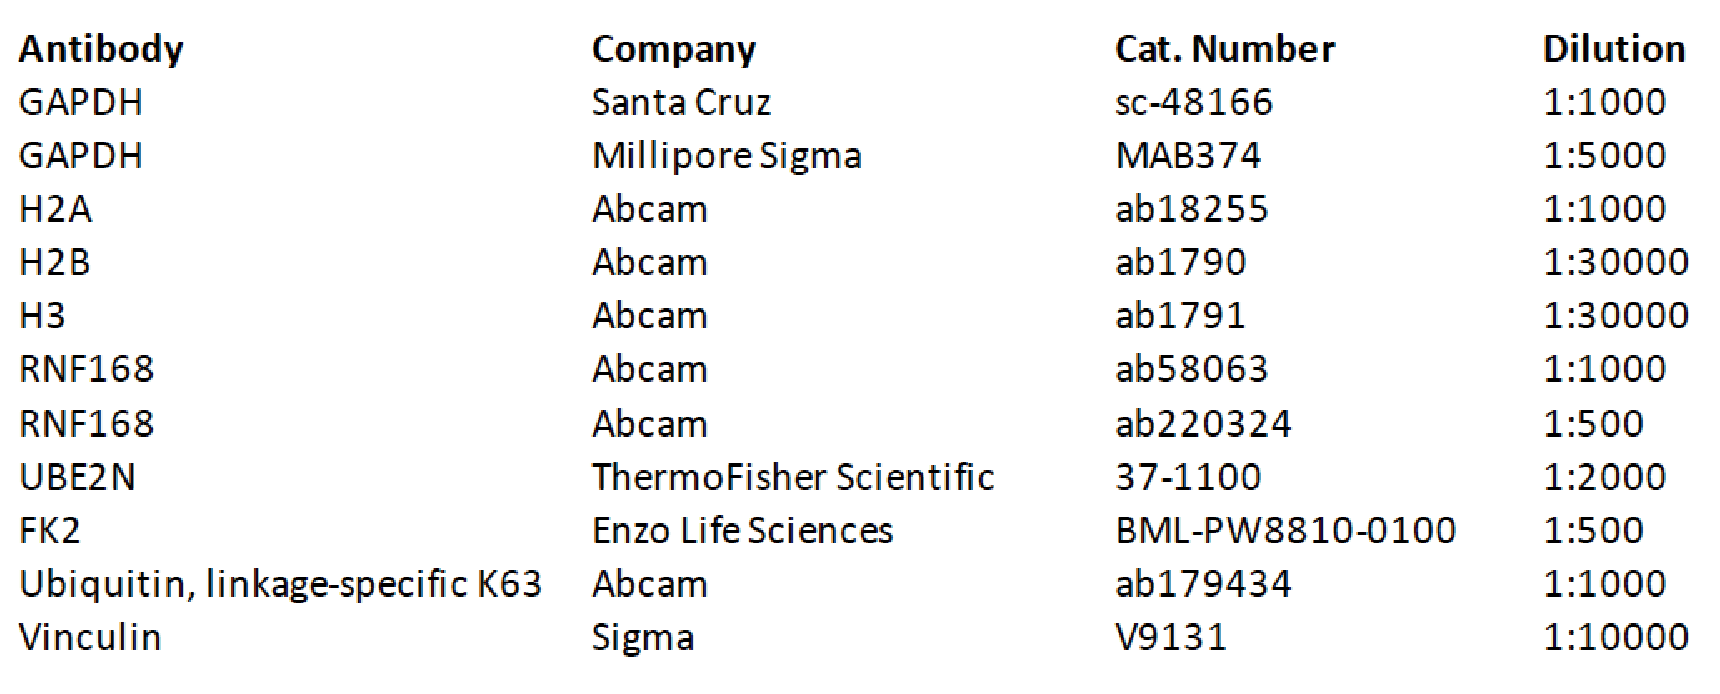
\includegraphics[width=1\textwidth]{supplement/tables/STable_Western_antibodies.png}
\label{table:Western_antibodies}
\end{table}
